% Author: Carles Marin (Claude, Anthropic, as AI research assistant).
% Part III. The centre charge returns: the even-m notch of the Wilson-line tower, the parity
% dichotomy, and why the two-Higgs fundamental domain does not transfer to the admissible class.
% Question-threaded narrative; honest about scope throughout. Build: pdflatex x2.
\documentclass[11pt,a4paper]{article}
\usepackage[utf8]{inputenc}
\usepackage{amsmath,amssymb,amsthm}
\usepackage{booktabs}
\usepackage[table,dvipsnames]{xcolor}
\usepackage{graphicx}
\usepackage{tikz}
\usetikzlibrary{shapes.geometric,arrows.meta,positioning,fit,backgrounds,patterns,calc}
\usepackage{geometry}
\geometry{margin=2.4cm}
\usepackage[colorlinks=true,linkcolor=RoyalBlue,citecolor=BrickRed,urlcolor=RoyalBlue]{hyperref}
\usepackage{caption}
\captionsetup{font=small,labelfont=bf}
\newtheorem{theorem}{Theorem}
\newtheorem{lemma}{Lemma}
\newtheorem{corollary}{Corollary}
\newcommand{\ZZ}{\mathbb{Z}}
\newcommand{\RR}{\mathbb{R}}
\newcommand{\su}[1]{SU(#1)}
\newcommand{\lam}{|\lambda|}
\definecolor{okgreen}{RGB}{0,140,54}
\definecolor{hdrblue}{RGB}{31,78,121}
\definecolor{softgrey}{RGB}{238,242,247}
\definecolor{warmred}{RGB}{178,34,34}

\title{\textbf{\Large A Centre-Charge Selection Rule\\ for the Wilson-Line Potential}\\[7pt]
\large\textnormal{\itshape The fundamental domain of gauge--Higgs unification\\
is representation-dependent}\\[8pt]
\normalsize\textnormal{Part III --- centre-parity selection, an exact decoupling,
and the gate we gave away}}
\author{Carles Mar\'in\thanks{Independent researcher, \texttt{karlesmarin@gmail.com}.
The computations were carried out and cross-checked with Claude (Anthropic) as an AI
research assistant against a common machine-verifiable ground truth (exact rational
arithmetic on $SU(n)$ weight systems in SageMath, and a \texttt{sorry}-free Lean~4
certificate for the central theorem); every number in this paper regenerates from the
ancillary scripts.}}
\date{\today\\[2pt]\small DOI: \href{https://doi.org/10.5281/zenodo.21438227}{10.5281/zenodo.21438227}}

\begin{document}
\maketitle

\begin{abstract}
\noindent
Part~II gave a gate away. Its first clause --- that a representation can display the
Standard Model's fractional hypercharges only if its $\ZZ_4$ centre charge $a+2b+3c$ is
odd --- was identified as the classical centre-charge congruence and disclaimed: \emph{we
claimed none of it}. This paper shows that the disclaimed gate is not a statement about
matter at all. It governs the Higgs sector, and for a reason that fits in one line:
\emph{advancing the Wilson line by one period is, up to a Weyl reflection, multiplication by
the central element $-\mathbf{1}\in Z(SU(4))$ --- and the centre charge is by definition how
a representation responds to one.} Writing $D(t)=\sum_{\text{weights}}
t^{\,n_2-n_4}(-1)^{n_3}$ for the signed generating function of the orbifold twist labels
--- a projection we \emph{derive} here from the $T^2/\ZZ_2$ boundary conditions rather than
import --- the character inherits the centre's response as
$D(-t)=(-1)^{a+2b+3c}D(t)$, and hence a dichotomy: a representation pairs its Kaluza--Klein
twist multiplicities at \emph{even} $m$ when the centre charge is odd, and at \emph{odd}
$m$ when it is even --- never both, except on a degenerate class $\mathcal Z$ that we
classify exactly and certify in Lean. The odd-$m$ case is not ours: it is the hypothesis
Akamatsu, Hirose, Maru and Nago verify by inspecting their Table~1 in order to halve the
Wilson-line fundamental domain to $\alpha_2\in[0,\tfrac12]$. Because Part~II's gate forces
the centre charge \emph{odd} for every representation that can host a quark generation,
while the gauge adjoint is unavoidably \emph{even}, the hypothesis inverts precisely on the
physical class: we verify directly that the potential of every admissible representation
violates period~$1$ in $\alpha_2$ by $2$--$30\%$ of its own scale, so the half-domain
reduction does not transfer and the full torus must be scanned. What the admissible class
gets instead is an exact decoupling: the notch annihilates the fermion representation's
entire contribution to the leading Kaluza--Klein order of the curvature at
$\alpha_2=\tfrac12$, leaving a gauge-only constant identical across all eight admissible
representations. The leading order is therefore degenerate \emph{by theorem}, every
distinction between candidate representations lives in subleading terms, and a naturalness
ranking built on point estimates is fragile for a structural reason rather than a numerical
one. We close by replacing the finite-difference Hessian with an integral measure of the
basin geometry, validated against it where it is trustworthy and stable where it is not.
Finally, the mechanism is neither an accident nor universal: the shift equals a central
element only when the Wilson-line-neutral slots carry balanced twist signs, which for a
single Wilson-line direction requires $N$ even --- so $SU(4)$ is the smallest group that can
carry this selection rule at all.
\end{abstract}

% ===================================================================
\section{The gate we gave away}\label{sec:intro}
This paper is about a sentence in its predecessor.

% MOVED-FIG1: placed early so the geometry precedes the roadmap
\begin{figure}[!t]
\centering
\resizebox{0.88\textwidth}{!}{%
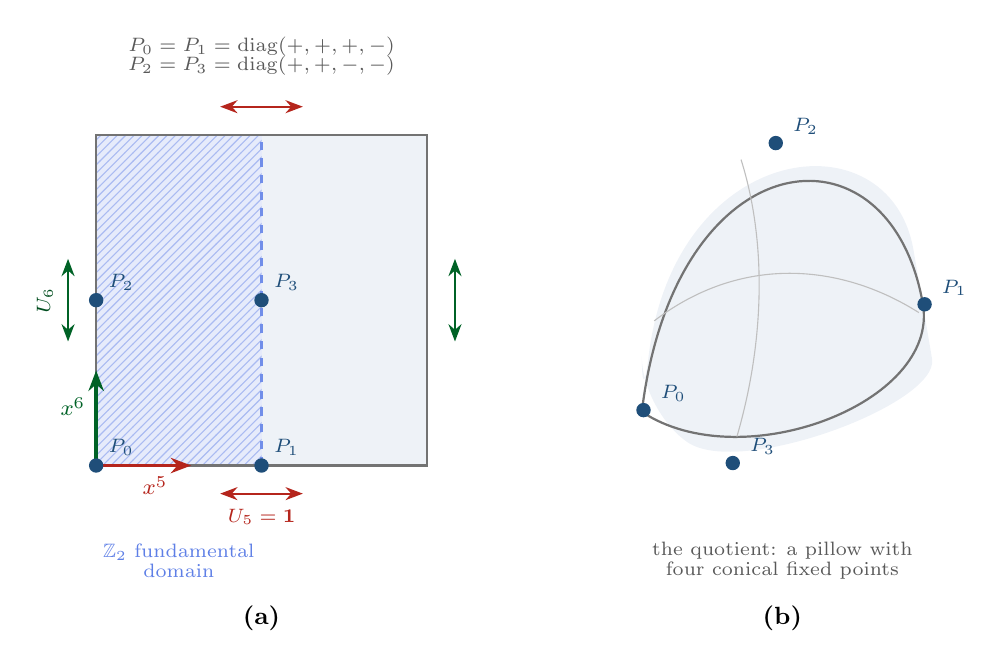
\begin{tikzpicture}[font=\small,x=1.05cm,y=1.05cm]
% ---------- (a) the flat fundamental domain ----------
\begin{scope}
\fill[softgrey] (0,0) rectangle (4,4);
\fill[RoyalBlue!13] (0,0) rectangle (2,4);
\draw[pattern=north east lines,pattern color=RoyalBlue!45,draw=none] (0,0) rectangle (2,4);
\draw[thick,black!55] (0,0) rectangle (4,4);
\draw[dashed,thick,RoyalBlue!75] (2,0) -- (2,4);
% basis vectors
\draw[-{Stealth[length=2.6mm]},very thick,BrickRed] (0,0) -- (1.15,0) node[below,pos=0.62,font=\footnotesize]{$x^5$};
\draw[-{Stealth[length=2.6mm]},very thick,okgreen!70!black] (0,0) -- (0,1.15) node[left,pos=0.62,font=\footnotesize]{$x^6$};
% edge identifications
\draw[{Stealth[length=2.2mm]}-{Stealth[length=2.2mm]},okgreen!70!black,thick] (-0.34,1.5) -- (-0.34,2.5);
\draw[{Stealth[length=2.2mm]}-{Stealth[length=2.2mm]},okgreen!70!black,thick] (4.34,1.5) -- (4.34,2.5);
\node[okgreen!55!black,font=\scriptsize,rotate=90] at (-0.62,2.0) {$U_6$};
\draw[{Stealth[length=2.2mm]}-{Stealth[length=2.2mm]},BrickRed,thick] (1.5,-0.34) -- (2.5,-0.34);
\draw[{Stealth[length=2.2mm]}-{Stealth[length=2.2mm]},BrickRed,thick] (1.5,4.34) -- (2.5,4.34);
\node[BrickRed,font=\scriptsize] at (2.0,-0.62) {$U_5=\mathbf{1}$};
% the four fixed points
\foreach \x/\y/\lb/\pv in {0/0/{P_0}/{(+,+,+,-)}, 0/2/{P_2}/{(+,+,-,-)},
                            2/0/{P_1}/{(+,+,+,-)}, 2/2/{P_3}/{(+,+,-,-)}}{
  \fill[hdrblue] (\x,\y) circle (2.6pt);
  \node[hdrblue,font=\scriptsize,above right=0pt and 1pt] at (\x,\y) {$\lb$};
}
\node[font=\scriptsize,black!65,align=center] at (2.0,4.95)
  {$P_0=P_1=\mathrm{diag}(+,+,+,-)$\\[-1pt]$P_2=P_3=\mathrm{diag}(+,+,-,-)$};
\node[RoyalBlue!85,font=\scriptsize,align=center] at (1.0,-1.15) {$\ZZ_2$ fundamental\\[-1pt]domain};
\node[font=\small\bfseries] at (2.0,-1.85) {(a)};
\end{scope}
% ---------- (b) the pillow ----------
\begin{scope}[shift={(6.6,0.35)}]
\fill[softgrey,rounded corners=20pt] (0,0.3) .. controls (0.4,3.6) and (3.0,3.9) .. (3.4,1.6)
   .. controls (3.6,0.4) and (1.2,-0.5) .. (0,0.3) -- cycle;
\draw[thick,black!55] (0,0.3) .. controls (0.4,3.6) and (3.0,3.9) .. (3.4,1.6)
   .. controls (3.6,0.4) and (1.2,-0.5) .. (0,0.3) -- cycle;
\draw[black!25,thin] (0.15,1.4) .. controls (1.2,2.2) and (2.4,2.1) .. (3.35,1.5);
\draw[black!25,thin] (1.15,0.0) .. controls (1.5,1.2) and (1.5,2.4) .. (1.2,3.35);
\foreach \x/\y/\lb in {0.02/0.32/{P_0}, 1.62/3.55/{P_2}, 3.42/1.6/{P_1}, 1.10/-0.32/{P_3}}{
  \fill[hdrblue] (\x,\y) circle (2.6pt);
  \node[hdrblue,font=\scriptsize,inner sep=2pt] at (\x+0.36,\y+0.20) {$\lb$};
}
\node[font=\scriptsize,black!65,align=center] at (1.7,-1.5) {the quotient: a pillow with\\[-1pt]four conical fixed points};
\node[font=\small\bfseries] at (1.7,-2.2) {(b)};
\end{scope}
\end{tikzpicture}}
\caption{\textbf{The geometry every later figure lives on.} \textbf{(a)} The torus $T^2$ with
the $\ZZ_2$ fundamental domain hatched. Translations around the two cycles are accompanied by
$U_5$ and $U_6$; inverting AHMN's consistency relations $P_1=U_5P_0$, $P_2=U_6P_0$ gives
$U_5=\mathbf{1}$ and $U_6=\mathrm{diag}(1,1,-1,1)$, which is the entire origin of the twist
label $q$ (\S\ref{sec:projection}). The four $\ZZ_2$ fixed points carry the parity matrices
shown; note $P_0=P_1$ and $P_2=P_3$, so only the $x^6$ direction carries a discrete twist ---
the asymmetry visible in \eqref{eq:twists}. \textbf{(b)} The quotient $T^2/\ZZ_2$: a pillow
with four conical points, one per fixed point. Every heatmap in this paper is the flat picture
of (a), drawn over the full period-$2$ range of the Wilson-line phases.}
\label{fig:fundamental}
\end{figure}

Part~I~\cite{PartI} took a question left open in 2003 --- Scrucca, Serone, Silvestrini and
Wulzer had observed that on an orbifold the cancellation of anomalies and the vanishing of
localized tadpoles are \emph{independent} requirements, and named the missing object an open
problem~\cite{SSSW} --- and met it inside the six-dimensional two-Higgs-doublet $SU(4)$
model of Akamatsu, Hirose, Maru and Nago~\cite{AHMN}: a coloured quark block in the
dimension-$60$ representation, a $45$-multiplet completion cancelling anomalies and tadpole
together, and an Existence theorem showing the tadpole never obstructs. Part~II~\cite{PartII}
turned the minimality that Part~I had merely observed into an exact law: an irreducible
$(a,b,c)$ of $SU(4)$ contains a Standard-Model quark cell among its $T^2/\ZZ_2$ chiral zero
modes if and only if
\begin{equation}\label{eq:criterion}
(a+2b+3c)\ \text{odd}\quad\wedge\quad b\ge1\quad\wedge\quad a+b+c\ge3 .
\end{equation}
Part~II was careful about credit, and nowhere more so than on the first clause. The $\ZZ_4$
centre charge --- Slansky's congruency class $c(R)=a+2b+3c \bmod 4$~\cite{Slansky} --- locks
fractional hypercharge to a fixed congruence, a fact stated for the Standard Model's own
$\ZZ_6$ by Hucks and by Saller and recast in global-structure language by Tong and by
Alonso, Dimakou and West~\cite{Hucks,Saller,Tong,Alonso}. Part~II wrote, in as many words,
\emph{``We claim none of it''}, and recorded the clause as \emph{inherited, not invented}.

Giving it away was the right call, and the reason is a long one. The observation that the
\emph{centre} of a gauge group carries physics the algebra alone does not goes back to
Dirac's quantization condition and was sharpened by 't~Hooft's classification of phases by
the electric and magnetic charges that survive it~\cite{tHooft}: what a theory permits as a
line operator, and what fractional charges it can carry, is decided not by
$\mathfrak{su}(n)$ but by which quotient of the simply connected group is gauged. Hucks and
Saller drew the corresponding conclusion for the Standard Model itself --- its true gauge
group is $\big(SU(3)\times SU(2)\times U(1)\big)/\ZZ_6$, and the familiar hypercharges
$\tfrac16,\tfrac23,-\tfrac13$ are precisely the fractions that quotient
permits~\cite{Hucks,Saller}. Tong recast the statement in the language of line
operators~\cite{Tong}, and Alonso, Dimakou and West asked the experimental question hiding
inside it --- which fractionally charged states would tell the candidate groups
apart~\cite{Alonso}. By the time Part~II needed the fact, it had been established four
separate times in four different languages. One does not claim such a thing.

That was correct, and this paper does not take it back. But it was incomplete in a way we
did not suspect, because it left a question unasked. The centre charge entered
\eqref{eq:criterion} as an \emph{arithmetic} condition on the matter sector: which weights
can carry $\tfrac16,\tfrac23,-\tfrac13$ at all. Nothing in that derivation suggests the same
congruence should have anything to say about the \emph{Higgs} sector --- about the
Wilson-line potential, its symmetries, its vacuum, or the mass it generates. The two live in
different parts of the construction and are computed from different data.

So: \emph{does the centre charge know anything about the Higgs potential?} The answer is that
it controls it, in a sense we can make exact. We do not claim the congruence. We claim what
it does --- and what it does is not a restriction on matter but a restriction on the
\emph{potential itself}.

\begin{center}
\fcolorbox{hdrblue}{RoyalBlue!6}{\parbox{0.94\textwidth}{%
\vspace{3pt}
\textbf{Centre-Parity Selection Principle.}\ \ Let a shift of a Wilson-line modulus be
Weyl-equivalent to multiplication by a central element $\zeta$ of order $d$. Then the Fourier
support of the one-loop potential splits into $d$ sectors labelled by the centre charge
modulo $d$, and a representation $R$ contributes to a sector only where
$\zeta^{\,c(R)}=1$. The sectors on which $\zeta^{\,c(R)}\neq1$ are \emph{identically empty} for
that representation --- not suppressed, absent.
\smallskip

\textbf{The case proved here} is $SU(4)$ on $T^2/\ZZ_2$, where $\zeta=-\mathbf{1}$ has $d=2$
and the charge is $c(R)=a+2b+3c$: one bit, read in four places ---
\emph{matter admissibility}, \emph{Kaluza--Klein twist pairing}, the \emph{Fourier support}
of the potential, and the \emph{geometry of its vacuum}.
\vspace{3pt}}}
\end{center}

\noindent
The centre charge has been used for half a century as a condition on which
\emph{representations} may carry fractional hypercharge; here it also decides which
\emph{harmonics} of the Hosotani potential can exist at all. Figure~\ref{fig:chain} draws
the centre of the group at the centre of the page, with the four sectors it governs around
it.

\begin{figure}[!t]
\centering
\begin{tikzpicture}[font=\small,
  pan/.style={rounded corners=3pt,draw,thick,align=center,inner sep=6pt,
              text width=3.45cm,fill=white,draw=black!35},
  ttl/.style={font=\footnotesize\bfseries},
  ray/.style={-{Stealth[length=2.6mm]},thick,black!45}]

% ---------------- the centre of the group, at the centre of the figure ----------------
\begin{scope}
\fill[RoyalBlue!6] (0,0) circle (2.22);
\draw[RoyalBlue!50,thick] (0,0) circle (1.90);
\foreach \a/\lb in {90/{1}, 0/{i}, 270/{-i}}
  {\fill[black!55] (\a:1.90) circle (2.2pt);
   \node[font=\scriptsize,black!55] at (\a:2.18) {$\lb$};}
\fill[BrickRed] (180:1.90) circle (3.6pt);
\node[font=\scriptsize\bfseries,BrickRed] at (180:2.30) {$-\mathbf{1}$};
% the half turn: one period of Wilson line
\draw[-{Stealth[length=2.6mm]},very thick,BrickRed] (84:1.90) arc (84:174:1.90);
\node[font=\scriptsize,BrickRed,align=center] at (0,2.70) {one period of $\alpha_2$};
% the answer, on a clean backing so nothing collides
\node[fill=white,rounded corners=2pt,inner sep=4pt,align=center,font=\scriptsize] at (0,0)
  {the centre\\[1pt]
   $Z\cong\ZZ_4$\\[4pt]
   answers with\\[1pt]
   $(-1)^{a+2b+3c}$\\[4pt]
   {\itshape one bit}};
\end{scope}

% ---------------- the four faces ----------------
% (1) matter
\node[pan] (p1) at (-5.0, 2.35)
  {\footnotesize\bfseries\ matter\\[3pt]
   \begin{tikzpicture}[scale=0.42,baseline]
     \draw[black!30] (-0.2,0)--(3.4,0);
     \foreach \x/\y/\lb in {0.35/1.10/{\tfrac23}, 1.75/0.28/{\tfrac16}, 3.15/-0.55/{-\tfrac13}}
       {\fill[RoyalBlue!75] (\x,\y) circle (5pt);
        \node[font=\tiny,above=1pt] at (\x,\y) {$\lb$};}
   \end{tikzpicture}\\[2pt]
   {\scriptsize which reps carry the SM fractions}\\[1pt]
   {\scriptsize\itshape Part~II \textperiodcentered\ classical}};
% (2) twist pairing
\node[pan] (p2) at (-5.0,-2.35)
  {\footnotesize\bfseries\ twist pairing\\[3pt]
   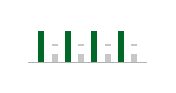
\begin{tikzpicture}[scale=0.42,baseline]
     \draw[black!30] (-0.1,0)--(3.5,0);
     \foreach \x in {0.3,1.1,1.9,2.7} \draw[okgreen!75!black,line width=2.2pt] (\x,0)--(\x,0.95);
     \foreach \x in {0.7,1.5,2.3,3.1} \draw[black!22,line width=2.2pt,dashed] (\x,0)--(\x,0.55);
   \end{tikzpicture}\\[2pt]
   {\scriptsize which comb of $(m,q)$ balances}\\[1pt]
   {\scriptsize\itshape \S\ref{sec:dichotomy}}};
% (3) Fourier support
\node[pan] (p3) at (5.0, 2.35)
  {\footnotesize\bfseries\ Fourier support\\[3pt]
   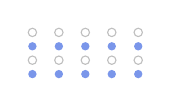
\begin{tikzpicture}[scale=0.42,baseline]
     \foreach \x in {0,...,4} \foreach \y in {0,...,3}
       {\pgfmathparse{int(mod(\y,2))}\ifnum\pgfmathresult=0
          \fill[RoyalBlue!70] (\x*0.8,\y*0.42) circle (3.6pt);
        \else
          \draw[black!25] (\x*0.8,\y*0.42) circle (3.6pt);
        \fi}
   \end{tikzpicture}\\[2pt]
   {\scriptsize which harmonics of $V$ may exist}\\[1pt]
   {\scriptsize\itshape \S\ref{sec:dichotomy} \textperiodcentered\ Fig.~\ref{fig:spectrum}}};
% (4) vacuum geometry
\node[pan] (p4) at (5.0,-2.35)
  {\footnotesize\bfseries\ vacuum geometry\\[3pt]
   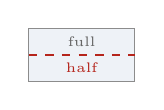
\begin{tikzpicture}[scale=0.42,baseline]
     \fill[softgrey] (0,0) rectangle (3.2,1.6);
     \draw[black!45] (0,0) rectangle (3.2,1.6);
     \draw[BrickRed,thick,dashed] (0,0.8)--(3.2,0.8);
     \node[font=\tiny,BrickRed] at (1.6,0.42) {half};
     \node[font=\tiny,black!60] at (1.6,1.2) {full};
   \end{tikzpicture}\\[2pt]
   {\scriptsize which domain must be scanned}\\[1pt]
   {\scriptsize\itshape \S\S\ref{sec:domain},\,\ref{sec:decoupling}}};

\foreach \p in {p1,p2,p3,p4} \draw[ray] (0,0) -- (\p);
\end{tikzpicture}
\caption{\textbf{The centre of the group, at the centre of the picture.} A period of the
Wilson line is a half turn of the $\ZZ_4$ centre --- it lands on $-\mathbf{1}$ --- and a
representation answers that element with the single bit $(-1)^{a+2b+3c}$. Everything this
paper proves is that bit read in four places: which representations may carry the
Standard-Model hypercharges (known, and disclaimed in Part~II), which comb of twist
multiplicities balances, which harmonics of the Wilson-line potential are allowed to be
non-zero at all, and how much of the torus must be searched for its vacuum. They look like
four separate facts about a model. They are one fact about a group.}
\label{fig:chain}
\end{figure}

\paragraph{Scope and relation to prior work.} As in Part~II we separate inherited from new,
and again most ingredients are inherited. The centre-charge congruence is
classical~\cite{Hucks,Saller,Tong,Alonso,Slansky}. The orbifold construction, the twist
labels $(m,q)$, the mass equation, the one-loop potential and the fundamental-domain
argument are all AHMN's~\cite{AHMN}; we quote their Section~4.3 verbatim in
\S\ref{sec:domain} because our central physical claim is about the reach of \emph{their}
hypothesis, not about an error in it --- their argument is correct for their model. The
mechanism behind our vanishing theorem is likewise classical: the alphabet
$\{1,-1,t,t^{-1}\}$ has determinant $-1$, so it parametrizes the improper component of
$O(4)$, where an irreducible representation and its associate $\mu\otimes\det$ have opposite
characters and self-associate ones vanish~\cite{Brauer}; the branching is Littlewood's
restriction rule with the Newell--King modification rules~\cite{King71,Newell,Brauer}, and
the determinant technique we use is described by Ayyer and Behrend as
routine~\cite{AyyerBehrend}. What is ours is fourfold: (i) the \emph{dichotomy}
(\S\ref{sec:dichotomy}) and the exact classification of its degenerate class
(\S\ref{sec:degenerate}), machine-certified in Lean~4; (ii) the observation --- with direct
verification --- that AHMN's fundamental-domain reduction \emph{inverts} on the
Standard-Model-admissible class (\S\ref{sec:domain}); (iii) the \emph{decoupling}
corollary and the resulting leading-order degeneracy (\S\ref{sec:decoupling}); and (iv) a
derivation of the $(m,q)$ projection from the boundary conditions (\S\ref{sec:projection}),
which in this construction had been used as a calibrated input. Figure~\ref{fig:roadmap} is
the route.

\emph{Established here:} the principle --- one period of Wilson line is a central gauge
transformation, so the centre charge is a statement about the potential and not only about
the matter. \emph{Left open:} all four of its readings, which are the rest of the paper.



\begin{figure}[t]
\centering
\resizebox{0.86\textwidth}{!}{%
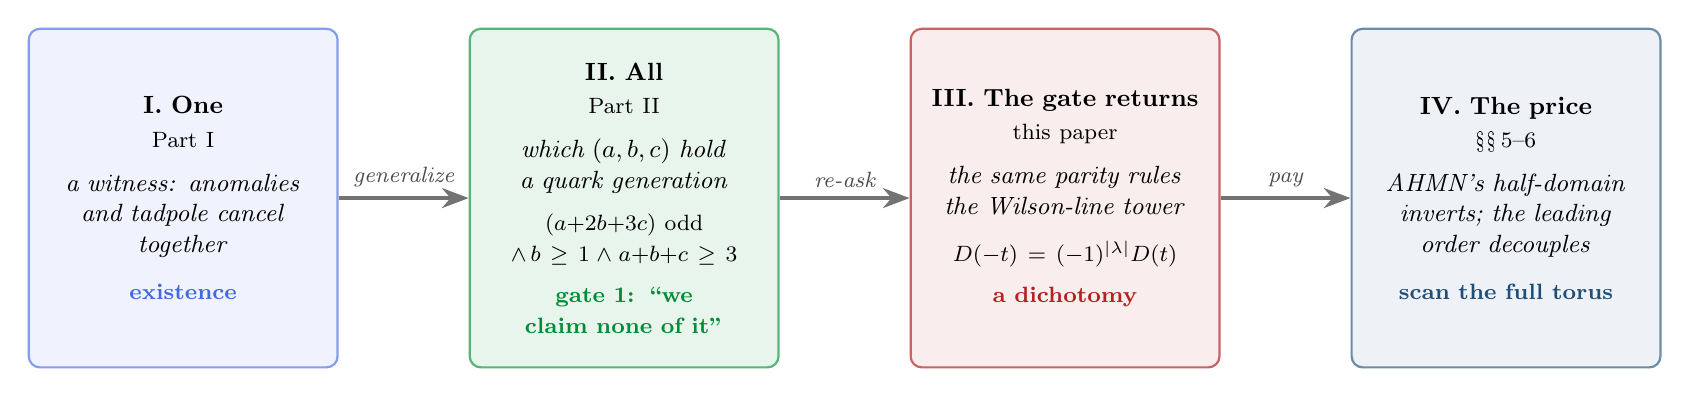
\begin{tikzpicture}[font=\small,
  act/.style={rounded corners,draw,thick,text width=3.5cm,align=center,inner sep=6pt,minimum height=4.3cm,anchor=north},
  arr/.style={-{Stealth[length=3.4mm]},very thick,black!55}]
\node[act,fill=RoyalBlue!8,draw=RoyalBlue!65] (a1) at (0,0)
 {\textbf{I.\ One}\\[1pt]{\footnotesize Part I}\\[5pt]
  \textit{a witness: anomalies}\\\textit{and tadpole cancel}\\\textit{together}\\[6pt]
  {\footnotesize\color{RoyalBlue}\textbf{existence}}};
\node[act,fill=okgreen!9,draw=okgreen!65] (a2) at (5.6,0)
 {\textbf{II.\ All}\\[1pt]{\footnotesize Part II}\\[5pt]
  \textit{which $(a,b,c)$ hold}\\\textit{a quark generation}\\[6pt]
  {\footnotesize$(a{+}2b{+}3c)$ odd\\$\wedge\,b\ge1\wedge a{+}b{+}c\ge3$}\\[4pt]
  {\footnotesize\color{okgreen}\textbf{gate 1: ``we claim none of it''}}};
\node[act,fill=warmred!8,draw=warmred!70] (a3) at (11.2,0)
 {\textbf{III.\ The gate returns}\\[1pt]{\footnotesize this paper}\\[5pt]
  \textit{the same parity rules}\\\textit{the Wilson-line tower}\\[6pt]
  {\footnotesize $D(-t)=(-1)^{\lam}D(t)$}\\[4pt]
  {\footnotesize\color{warmred}\textbf{a dichotomy}}};
\node[act,fill=softgrey,draw=hdrblue!65] (a4) at (16.8,0)
 {\textbf{IV.\ The price}\\[1pt]{\footnotesize \S\S\,5--6}\\[5pt]
  \textit{AHMN's half-domain}\\\textit{inverts; the leading}\\\textit{order decouples}\\[6pt]
  {\footnotesize\color{hdrblue}\textbf{scan the full torus}}};
\draw[arr] (a1.east) -- node[above,font=\footnotesize\itshape,black!70]{generalize} (a2.west);
\draw[arr] (a2.east) -- node[above,font=\footnotesize\itshape,black!70]{re-ask} (a3.west);
\draw[arr] (a3.east) -- node[above,font=\footnotesize\itshape,black!70]{pay} (a4.west);
\end{tikzpicture}}
\caption{The arc of the series. Part~I produced a single consistent model; Part~II the exact
law of which representations are eligible, explicitly disclaiming its arithmetic gate as
classical. This paper asks what that disclaimed gate does elsewhere, and finds it governing
the gauge--Higgs potential --- with a consequence that must be paid before any
vacuum in this class is computed.}
\label{fig:roadmap}
\end{figure}

% ===================================================================
\section{Where the twist labels come from}\label{sec:projection}
Before anything can be proved about the tower, one has to know exactly what labels it.

The labels are old. In 1979 Scherk and Schwarz noticed that a field on a compact space need
not come back to itself: it may return acted on by a symmetry, and the resulting twist gives
masses that no potential put there~\cite{ScherkSchwarz}. In the same year Manton and Fairlie
observed that the extra-dimensional components of a gauge field are scalars in four
dimensions, with a quartic coupling fixed by the gauge coupling rather than
free~\cite{Manton,Fairlie}; Hosotani then showed that the vacuum of such a scalar is a
Wilson line, so that symmetry breaking becomes a statement about holonomy around a
cycle~\cite{Hosotani}. That is the whole idea of gauge--Higgs unification: the Higgs is a
twist. Orbifolds entered when Kawamura used a $\ZZ_2$ projection to split a
grand-unified multiplet~\cite{KawamuraGUT}, and the modern constructions --- AHMN's
included --- combine the two, so that a mode carries \emph{both} a Wilson-line phase and a
discrete parity. That pair of data is exactly what $(m,q)$ records.

Which is why the pair has to be pinned down before anything else. AHMN
attach to each Kaluza--Klein mode a pair of integers $(m,q)$ through twisted boundary
conditions~\cite[Eqs.~(3.3)--(3.4)]{AHMN},
\begin{equation}\label{eq:twists}
f(x^5+2\pi R,x^6)=e^{i\pi m\alpha_1}f(x^5,x^6),\qquad
f(x^5,x^6+2\pi R)=e^{i\pi(m\alpha_2+q)}f(x^5,x^6),
\end{equation}
with $\alpha_{1,2}=gRv_{1,2}$ the Wilson-line phases, $m$ ``the weight of the generator'' and
$q\in\{0,1\}$ periodic or antiperiodic. In terms of the partition coordinates
$n=(n_1,n_2,n_3,n_4)$ of a weight this construction is used with $m=n_2-n_4$ and
$q=n_3\bmod2$. That assignment is usually justified by checking it against AHMN's Table~1.
Checking is not deriving, so we derive it.

The boundary data are AHMN's, and Figure~\ref{fig:fundamental} collects them --- translations
$U_{5,6}$, parities $P_i$ at the four fixed
points, and the consistency relations $P_1=U_5P_0$, $P_2=U_6P_0$~\cite[Eq.~(2.8)]{AHMN},
with the choice~\cite[Eqs.~(2.9)--(2.10)]{AHMN}
\[
P_0=P_1=\mathrm{diag}(+,+,+,-),\qquad P_2=P_3=\mathrm{diag}(+,+,-,-),
\]
which breaks $SU(4)\to SU(2)_L\times U(1)_Y\times U(1)_X$. Inverting the relations,
\begin{equation}\label{eq:U}
U_5=P_1P_0^{-1}=\mathbf{1},\qquad
\boxed{\,U_6=P_2P_0^{-1}=\mathrm{diag}(1,1,-1,1)\,}
\end{equation}
A state of content $n$ in any tensor representation therefore picks up
$\prod_i (U_6)_{ii}^{\,n_i}=(-1)^{n_3}$ under the $x^6$ translation, which is exactly the
periodic/antiperiodic alternative in \eqref{eq:twists}: $q=n_3\bmod2$. Two independent
checks come for free. First, $q$ is not an extra datum but the \emph{product of the two
$\ZZ_2$ parities}: on content $n$, $P_0\mapsto(-1)^{n_4}$ and $P_2\mapsto(-1)^{n_3+n_4}$,
whose product is $(-1)^{n_3}$, consistent with $U_6=P_2P_0$. Second, and more tellingly,
\eqref{eq:twists} is \emph{asymmetric} --- the $x^5$ condition carries no $q$ and the $x^6$
condition does. AHMN do not comment on this. It is precisely $U_5=\mathbf{1}$ against
$U_6\neq\mathbf{1}$: there is no discrete twist along $x^5$ for a $q$ to describe.

For $m$: the components of $A_{5,6}$ with four-dimensional massless modes --- the $(++)$
entries of~\cite[Eq.~(2.12)]{AHMN} --- sit at matrix positions $(1,4),(2,4),(4,1),(4,2)$,
which are the two Higgs doublets. The Wilson-line vacuum expectation values lie there, and
using $SU(2)_L$ (acting on indices $1,2$) to align with the second doublet component makes
the generator $E_{24}+E_{42}$, conjugate inside the $\{2,4\}$ block to
\begin{equation}
T=\mathrm{diag}(0,1,0,-1),
\end{equation}
whose weight on content $n$ is $n_2-n_4$. That a \emph{single} $m$ appears in both halves of
\eqref{eq:twists} is consistent: both cycles carry the same Lie-algebra direction with
different magnitudes $v_1,v_2$. The choice of index pair is $SU(2)_L$ gauge freedom, and it
is provably immaterial --- the generating function $D$ of \S\ref{sec:dichotomy} is invariant
under all $24$ assignments $m=n_i-n_j$, $q=n_k\bmod2$ with $i,j,k$ distinct. The freedom in
the derivation and the freedom in the theorem are the same freedom.

\paragraph{Reading AHMN's Table~1 correctly.} Applying $(T,U_6)$ to the $\mathbf{35}=(4,0,0)$ gives,
for $m\ge1$, the counts $3,3,3,1,1,1,1$ at $(1,0),(1,1),(2,0),(2,1),(3,0),(3,1),(4,0)$,
matching AHMN's Table~1 entry by entry --- but as counts of $SU(2)_L$ \emph{multiplets},
not of states. The reason is physical. $T$ does not commute with $SU(2)_L$: moving a box
between indices $1$ and $2$ shifts $n_2$, hence $m$, by one. A multiplet of size $s$
therefore does not carry a single $m$; it spreads over $s$ \emph{consecutive} values,
contributing exactly one state to each. We verify this on the $\mathbf{35}$ with no
exceptions, and the identity ``\#weights at $(m,q)$ $=$ \#multiplets spanning $(m,q)$'' holds
exactly. That the Wilson line splits $SU(2)_L$ multiplets is not bookkeeping --- it is
electroweak symmetry breaking, which is what the Wilson line is for.

\emph{Established here:} $q$ is the $U_6=P_2P_0^{-1}$ twist, equivalently the product of the
two orbifold parities, and $m$ is the weight under the Wilson-line generator; AHMN's
Table~1 is reproduced \emph{and} explained. \emph{Left open:} nothing at this level --- what remains an
input is AHMN's parity choice itself, which is their model definition, as it should be.

% ===================================================================
\section{Centre-parity selection, and the dichotomy it forces}\label{sec:dichotomy}
With the labels fixed we can ask a sharp question about the tower --- and the way to ask it
is itself borrowed.

There is a long habit in representation theory of learning about a character by evaluating
it at a \emph{distinguished} group element rather than studying it in general. Weyl's
\emph{Classical Groups} is built on the technique~\cite{Weyl}, and Littlewood turned it into
a machine: feed a Schur function an alphabet with structure --- variables in $\pm$ pairs,
say --- and the answer is not merely simpler but combinatorial, vanishing outright unless
the partition passes a divisibility test~\cite{LittlewoodBook}. The habit is very much
alive: Ciucu and Krattenthaler found that characters at reciprocal pairs
$x,x^{-1}$ factorize~\cite{CiucuKrattenthaler}, Ayyer and Behrend widened the
class~\cite{AyyerBehrend}, and Ayyer and Kumari classified exactly which partitions survive
a root-of-unity twist~\cite{AyyerKumari,Kumari}. In every case the special element converts
a question about representations into arithmetic on a Young diagram.

Our tower hands us such an element for free. The two orbifold parities and the Wilson line
together evaluate the $SU(4)$ character at an alphabet that is half $\pm1$ and half
reciprocal --- and, as we will see, that alphabet is not a convenient choice but the one the
physics dictates. So we follow the habit. Define the signed generating function of the twist
labels,
\begin{equation}\label{eq:D}
D(t)\;=\;\sum_{\text{weights}} t^{\,n_2-n_4}\,(-1)^{n_3}\;=\;s_\lambda\!\left(1,-1,t,t^{-1}\right),
\qquad \lambda=(a{+}b{+}c,\;b{+}c,\;c,\;0),
\end{equation}
the second equality because $s_\lambda(x)=\sum_{\text{weights}}\prod_i x_i^{n_i}$ evaluated
at $x=(1,t,-1,t^{-1})$, reordered by symmetry. Since the $(m,q)$ classes partition the
weights and $(-1)^{n_3}$ is constant on each,
\begin{equation}
[t^m]\,D(t)\;=\;\mathrm{mult}(m,0)-\mathrm{mult}(m,1),
\end{equation}
so $D$ records exactly the failure of the two twist sectors to balance, level by level.
Call $(a,b,c)$ \emph{even-notched} if $\mathrm{mult}(m,0)=\mathrm{mult}(m,1)$ for every even
$m$, and \emph{odd-notched} if the same holds for every odd $m$. The first happens iff $D$ is
an odd Laurent polynomial, the second iff $D$ is even.

\paragraph{How this was found, since it matters for how much to trust it.} The lemma below
is two lines, which makes it look like the sort of thing one writes down first and then goes
looking for an application. That is not what happened, and the actual order is worth
recording because it is the same order Part~I recommended: notice a regularity, then ask
whether it is a law.

The even-$m$ notch appeared first as an \emph{empirical} oddity. Tabulating $(m,q)$
multiplicities across the admissible catalogue while working on something else, we noticed
that every admissible representation balanced its even-$m$ levels exactly, and that AHMN's
$\mathbf{35}$ --- the one representation in the table that cannot host a quark generation ---
did not, missing by $3$ against $1$ at $m=2$. Eight cases and one exception is a pattern, not
a theorem, and our first explanation for it was wrong: we conjectured the responsible clause
was Part~II's second gate, $b\ge1$, and falsified it within the hour on the explicit
counterexamples $(2,1,0)$ and $(0,2,0)$, which have $b\ge1$ and no notch. Only after that
failure did we look for the invariant that the parity of the centre charge supplies, and only
then did the two-line proof exist to be written. The classification of the degenerate class
in \S\ref{sec:degenerate} came later still, forced by the cases the lemma leaves open. We
record the sequence because a reader is entitled to know whether a clean statement was
reverse-engineered from a clean proof or extracted from messy data; this one came from the
data, and the counterexamples that killed the first attempt are in the ancillary scripts
alongside the ones that confirm the second.

\begin{lemma}[Parity]\label{lem:parity}
$D(-t)=(-1)^{\lam}D(t)$, with $\lam=a+2b+3c$ the number of boxes of $\lambda$.
\end{lemma}
\begin{proof}
As multisets $\{1,-t,-1,-t^{-1}\}=-\{1,t,-1,t^{-1}\}$; $s_\lambda$ is symmetric and
homogeneous of degree $\lam$.
\end{proof}

\paragraph{The principle: a unit shift of the Wilson line is a central gauge transformation.}
Written that way the lemma looks like an accident of Schur functions, and it is worth saying
plainly why it is not --- because the reason is the whole content of this paper.

The generating variable tracks the twist level, $t^m\leftrightarrow e^{i\pi m\alpha_2}$, so
$t\to-t$ is nothing other than $\alpha_2\to\alpha_2+1$: one unit of Wilson line. Write
$g(\alpha_2)$ for the group element the orbifold hands us --- the $U_6$ twist times the
Wilson line, with eigenvalues $(1,\,t,\,-1,\,t^{-1})$ in the slots of \S\ref{sec:projection}.
Then

\[
\begin{aligned}
g(\alpha_2{+}1)\ &=\ \mathrm{diag}\big(\,1,\ -t,\ -1,\ -t^{-1}\big),\\[2pt]
(-\mathbf{1})\cdot g(\alpha_2)\ &=\ \mathrm{diag}\big(-1,\ -t,\ \ \,1,\ -t^{-1}\big).
\end{aligned}
\]

These are \emph{not} the same matrix, and we are careful not to say they are: the shift on its
own, $\mathrm{diag}(1,-1,1,-1)$, is not central. They agree \emph{up to a Weyl element}, the
unique permutation relating them being the transposition of slots $1$ and $3$. That is
enough, because a character is a class function:

\begin{equation}\label{eq:principle}
\boxed{\ g(\alpha_2{+}1)\ \sim_{W}\ (-\mathbf{1})\cdot g(\alpha_2),
\qquad -\mathbf{1}\in Z\big(SU(4)\big)\cong\ZZ_4 .\ }
\end{equation}

The centre of $SU(4)$ is $\{\zeta\mathbf{1}:\zeta^4=1\}$, and $-\mathbf{1}$ is its unique
element of order two ($\det(-\mathbf{1})=(-1)^4=1$, so it does lie in $SU(4)$). On an
irreducible representation $\zeta\mathbf{1}$ acts by the scalar $\zeta^{\lam}$ --- that is
what the $n$-ality \emph{is} --- so $-\mathbf{1}$ acts by $(-1)^{\lam}$, and
$\chi_\lambda(g(\alpha_2{+}1))=(-1)^{\lam}\chi_\lambda(g(\alpha_2))$. That is the parity
lemma, and \eqref{eq:principle} is why it had to hold:

\begin{quote}
\emph{Advancing the Wilson line by one period is, up to a Weyl reflection, a central gauge
transformation --- and the centre charge is by definition how a representation responds to
one.}
\end{quote}

The Weyl element is not a technicality to be apologised for; it is where the orbifold enters.
The permutation that does the job exchanges the \emph{free} slot, where the alphabet is $+1$,
with the slot carrying the $U_6$ twist, where it is $-1$. Without that twist there would be
no $-1$ in the alphabet to pair with the $+1$, the negation could not be undone by any
permutation, and no selection rule would exist. The same $U_6$ that produces the label $q$ in
\S\ref{sec:projection} is what makes the centre charge visible to the potential at all.

Two consequences are worth stating before the details. First, nothing here is special to
Schur functions: in any construction where a shift of a modulus realizes a central element up
to Weyl, a centre-charge selection rule follows, whether or not anyone has written it down.
Second, the \emph{mechanism} is not special to $SU(4)$ either --- every $SU(N)$ has a centre
$\ZZ_N$ --- but the \emph{congruence} that appears is: it is fixed by the order of the
central element the shift realizes, which is two here and need not be elsewhere.
\S\ref{sec:reflections} takes that up, since it is the first question a reader should ask.

The lemma itself is elementary, and we present it as bookkeeping rather than as a result.
Its consequence is not.

\begin{corollary}[Dichotomy]\label{cor:dichotomy}
Every irreducible representation of $SU(4)$ is even-notched or odd-notched, and not both,
except on the degenerate class $D\equiv0$ where it is both:
\[
\lam\ \text{odd}\ \Longrightarrow\ \text{pairing at \textbf{even} }m,\qquad
\lam\ \text{even}\ \Longrightarrow\ \text{pairing at \textbf{odd} }m .
\]
\end{corollary}

\begin{figure}[t]
\centering
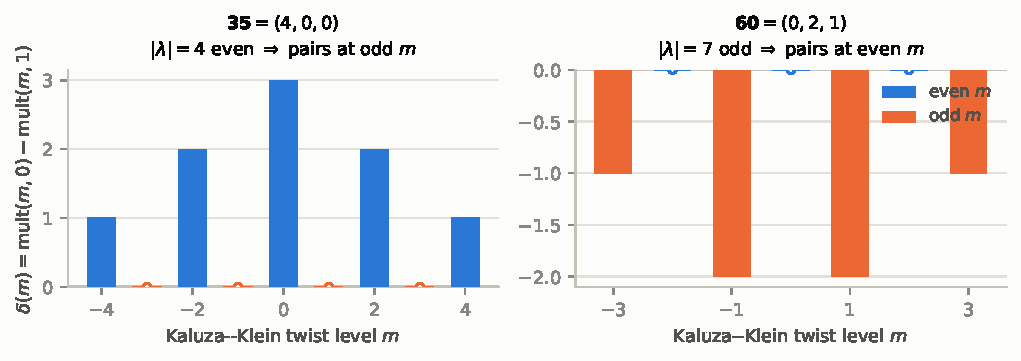
\includegraphics[width=\textwidth]{fig_combs.pdf}
\caption{The dichotomy, seen directly. The signed imbalance
$\delta(m)=\mathrm{mult}(m,0)-\mathrm{mult}(m,1)$ for AHMN's fermion (left) and for the
smallest representation able to host a quark generation (right). Each is a \emph{comb}: one
vanishes on every even tooth, the other on every odd one, and which comb a representation
gets is decided by a single bit, the parity of its centre charge. Hollow markers sit on the
teeth that vanish identically. No representation has both combs full, and outside the class
$\mathcal Z$ of \S\ref{sec:degenerate} none has both empty.}
\label{fig:combs}
\end{figure}

Figure~\ref{fig:combs} is the corollary with the algebra taken out. Two remarks fix the
meaning. First, $\lam=a+2b+3c\equiv a+c \pmod 2$, so the parity in
question is Part~II's gate~1 exactly --- and it is the $\ZZ_2$ \emph{quotient} of the $\ZZ_4$
centre charge, not the centre charge itself. Second, the same parity was already doing silent
work in Part~II: the chiral zero-mode count $N=(b+1)(a+c+1)/2$ is an integer only because
$a+c$ is odd whenever the centre charge is odd, a parenthetical remark there. Three
appearances, in three sectors that share no coordinate: the admissibility gate, the
integrality of the zero-mode count, and now the tower's twist balance. It is the invariant
doing the work, not the frame.

\paragraph{The notch is a hole, not a cancellation.} It is worth seeing what
Corollary~\ref{cor:dichotomy} does to the potential itself, because the statement is more
concrete than ``multiplicities balance''. Expanding $V$ in Fourier modes on the torus, the
amplitude at the frequency vector $m\,(k_1,k_2)$ --- the $m$-th harmonic along the
direction $(k_1,k_2)$ --- carries the factor
$\sum_q\mathrm{mult}(m,q)\,(-1)^{k_2q}$, which is the \emph{total} multiplicity when $k_2$ is
even and exactly $\delta(m)$ when $k_2$ is odd. The notch therefore does not arrange a
delicate cancellation among contributions: it empties an entire sublattice of Fourier space.
For a representation of odd centre charge, \emph{every} mode with $k_2$ odd and $m$ even is
identically absent from the potential --- not small, absent. Figure~\ref{fig:spectrum} shows
the eight admissible representations leaving precisely the same seats vacant, and AHMN's
$\mathbf{35}$ filling all $95$ of them.

\begin{figure}[p]
\centering
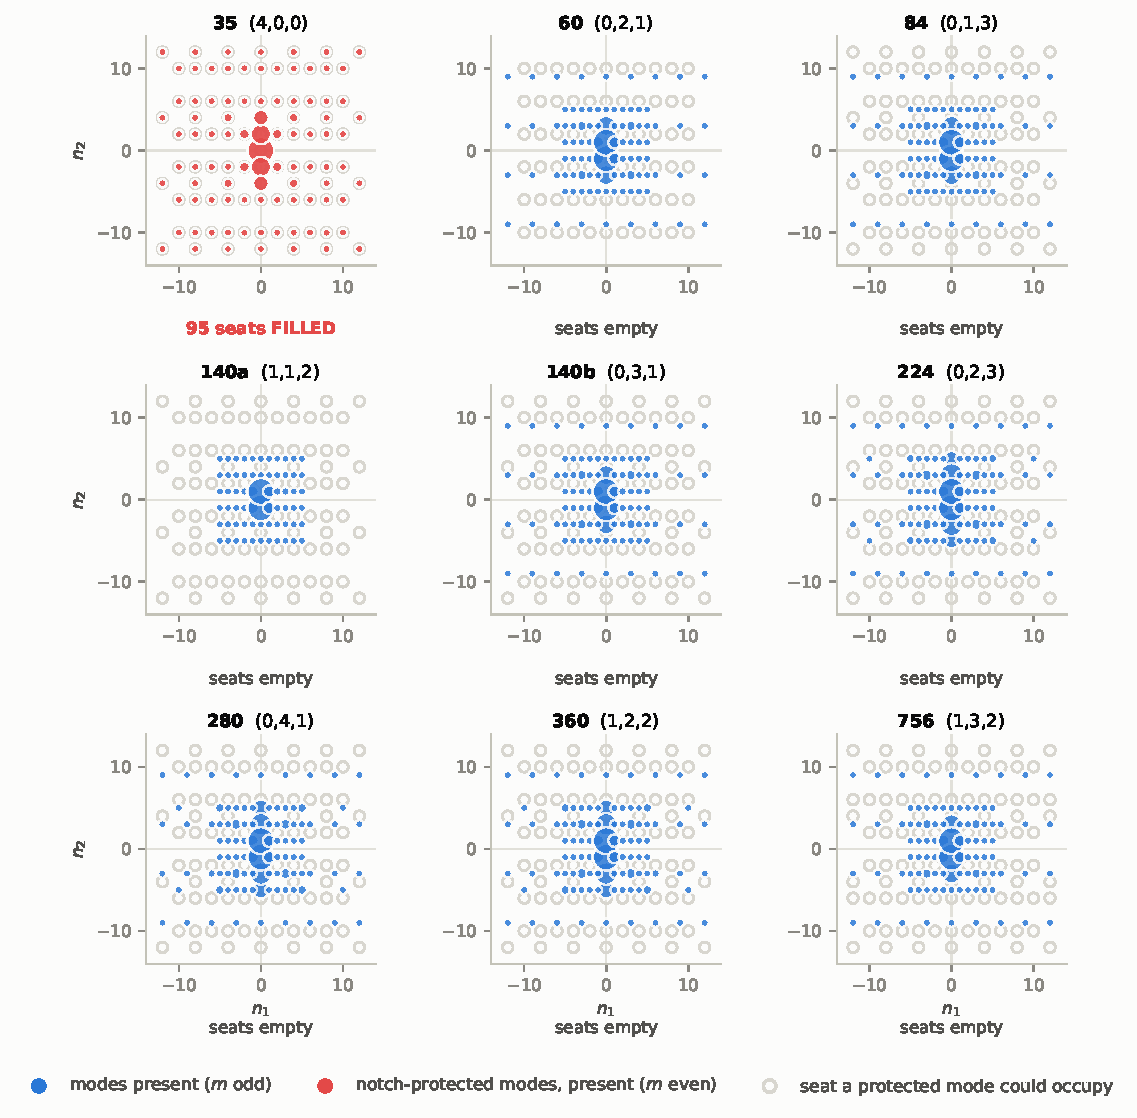
\includegraphics[width=0.93\textwidth]{fig_spectrum.pdf}
\caption{\textbf{The notch, seen as absence.} Each panel is the Fourier plane of the
one-loop potential for one representation, restricted to the odd-$k_2$ shells --- the sector
whose amplitude is $\delta(m)$. Filled discs are modes the potential actually carries, sized
by amplitude; hollow rings mark every seat a \emph{notch-protected} mode ($m$ even) could
occupy. Eight representations leave all of those seats empty, and they are exactly the eight
that can host a Standard-Model quark generation. The ninth, AHMN's $\mathbf{35}$, fills
them. Nothing was fitted or thresholded: the empty seats are exact zeros, and the pattern is
the single bit $a{+}2b{+}3c \bmod 2$ made visible.}
\label{fig:spectrum}
\end{figure}

\emph{Established here:} exactly one of the two pairings holds, which one is decided by
the centre charge's parity, and the consequence is an identically empty sublattice of the
potential's Fourier support. \emph{Left open:} the degenerate class where both hold, and ---
the point of the paper --- what the odd-$m$ case is doing in the literature already.

% ===================================================================
\section{The degenerate class}\label{sec:degenerate}
Corollary~\ref{cor:dichotomy} is silent when $D$ vanishes identically. That class is small,
exactly computable --- and its existence is the fingerprint of a group that is not connected.

$O(n)$ has two components, and everything awkward about its representation theory descends
from that. Its irreducible representations come in \emph{associate} pairs $\mu$ and
$\mu\otimes\det$, indistinguishable on the rotations and opposite on the reflections; some
are their own partner. Because Young diagrams were built for $GL$ and $S_n$, labelling
$O(n)$ representations by them produces ``non-standard'' labels that must be repaired, and
Newell wrote the repair rules in 1951~\cite{Newell}, with King systematizing them for all
three classical families two decades later~\cite{King71}. The awkwardness is not
bookkeeping fussiness; it is the disconnectedness showing through the notation. Koike and
Terada's influential reformulation resolves it in the cleanest possible way --- by working
in $R(SO(n))$ and treating the $O(n)$ labels as a basis~\cite{KoikeTerada} --- which is
elegant, universally used, and, for our purposes, precisely the wrong move: identifying
$\mu$ with $\mu\otimes\det$ is exactly the information we need.

That is the sense in which the class below exists. It consists of the representations whose
branching is \emph{blind} to the reflection --- self-associate through and through, so that
every contribution cancels against a partner. The physics saw it first, as a tower with
both combs empty.

\begin{theorem}[Degenerate class]\label{thm:Z}
$D\equiv0$ if and only if
\[
\boxed{\;b\ \text{odd}\ \wedge\ \big[(a,c\ \text{both odd})\ \vee\ (a=c\ \text{even})\big]\;}
\]
Consequently the even-$m$ notch holds iff $a+2b+3c$ is odd or $(a,b,c)\in\mathcal Z$, and
since every member of $\mathcal Z$ has $\lam$ even, $\mathcal Z$ is disjoint from the class
satisfying Part~II's gate.
\end{theorem}

\begin{proof}[Proof sketch]
Write $D=N/V$ with $N=\det(y_i^{\mu_j})$ the bialternant on the ordered alphabet
$y=(1,-1,t,t^{-1})$ and $\mu=(a{+}b{+}c{+}3,\;b{+}c{+}2,\;c{+}1,\;0)$. Laplace-expand $N$
along the two \emph{constant} rows: the $2\times2$ minor on columns $j<k$ is
$(-1)^{\mu_k}-(-1)^{\mu_j}$, so only columns of opposite $\mu$-parity survive, while every
complementary minor on the rows $(t,t^{-1})$ equals $[\mu_l-\mu_m]$ with
$[x]:=t^x-t^{-x}$. The eight parity classes of $(a,b,c)$ fall into four types. If all $\mu_j$
are even --- that is, $a,b,c$ all odd --- every surviving minor vanishes and $N\equiv0$. If
exactly one $\mu_j$ has the minority parity, $N$ is a combination of three brackets whose
largest argument is the sum of the other two, hence cannot cancel. Of the three classes with
a two-two parity split, two contain the bracket $[P]$ with $P=a{+}b{+}c{+}3$ strictly larger
than every other argument, so again no cancellation; the third, $a,c$ even and $b$ odd, gives
$N/2=[Q]-[R]+[P{-}Q]-[P{-}R]$ with all four arguments positive, which vanishes iff
$\{Q,P{-}Q\}=\{R,P{-}R\}$ as multisets, and since $Q=R$ would force $b=-1$ this happens iff
$a=c$. The only analytic input is that $\{[x]\}_{x>0}$ is linearly independent, which is the
statement that distinct monomials are independent.
\end{proof}

The theorem is verified four independent ways --- Weyl weight multiplicities, an exact
bialternant sweep over $10\,648$ representations to $(a,b,c)\le21$ with no mismatch, symbolic
checks of each case formula, and an adversarial audit --- and certified in Lean~4
(Table~\ref{tab:lean}). Figure~\ref{fig:landscape} puts the theorem and Part~II's criterion on
the same plate: $\mathcal Z$ occupies its own cells and never meets a representation able to
host a quark generation, which is Corollary~\ref{cor:dichotomy}'s disjointness seen rather
than deduced.

\begin{figure}[t]
\centering
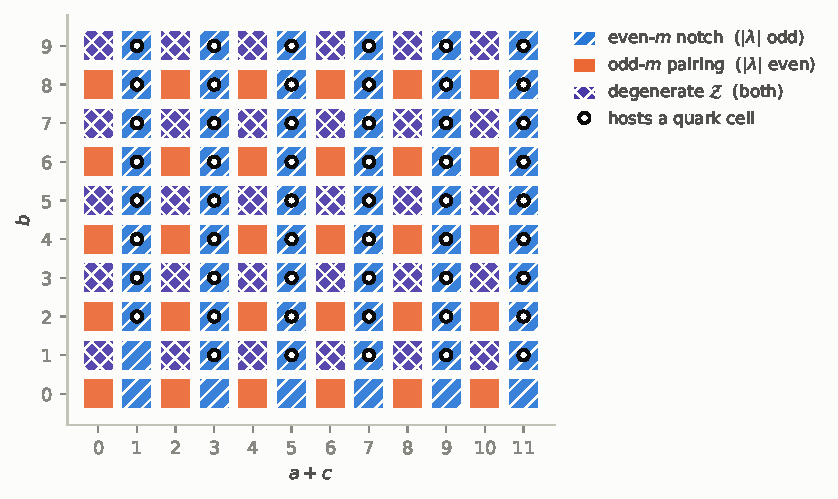
\includegraphics[width=0.92\textwidth]{fig_landscape_notch.pdf}
\caption{The whole landscape on one plate. Each cell is a label pair $(a+c,\,b)$ --- the two
coordinates the classification actually depends on --- coloured by which pairing the tower
satisfies. The blue column-parity is Part~II's gate~1 in disguise: those are precisely the
representations that can host a quark generation, ringed where the remaining two clauses
($b\ge1$, $a+b+c\ge3$) also hold. Violet cells are the degenerate class $\mathcal Z$ of
Theorem~\ref{thm:Z}, which satisfies both pairings and, as the figure makes visible, never
touches a ring. Everything in this paper is a statement about the boundary between the blue
and the orange.}
\label{fig:landscape}
\end{figure}

\begin{table}[t]
\centering\small
\begin{tabular}{p{5.7cm}p{8.4cm}}
\toprule
\rowcolor{hdrblue}
\textcolor{white}{Lean theorem (\texttt{NotchCentreCharge.lean})} & \textcolor{white}{content}\\
\midrule
\texttt{notch\_degenerate\_iff} &
$N\,a\,b\,c=0 \leftrightarrow (\mathrm{Odd}\,b \wedge ((\mathrm{Odd}\,a\wedge \mathrm{Odd}\,c)\vee a=c))$ --- Theorem~\ref{thm:Z}, over
$\ZZ[T;T^{-1}]$, no \texttt{decide} on the determinant\\
\midrule
\rowcolor{softgrey}
\texttt{notch\_parity} &
Lemma~\ref{lem:parity} as a division-free identity on the bialternant\\
\midrule
\texttt{degenerate\_centre\_charge\_even} &
every member of $\mathcal Z$ has $a+2b+3c$ even\\
\midrule
\rowcolor{softgrey}
\texttt{degenerate\_disjoint\_admissible} &
$\lam$ odd $\Rightarrow N\neq0$; the two classes never meet\\
\bottomrule
\end{tabular}
\caption{The machine-checked core. All statements are \texttt{sorry}-free and depend only on
\texttt{propext}, \texttt{Classical.choice}, \texttt{Quot.sound}. The linear-independence step
is replaced by extraction of a single Laurent coefficient at the strictly largest bracket
argument, which is finite and effective.}
\label{tab:lean}
\end{table}

\paragraph{What is new here, and what is not.} The mechanism is classical and we state it
plainly. The alphabet $\{1,-1,t,t^{-1}\}$ has determinant $-1$, so it is the generic
semisimple element of the \emph{improper} component $O(4)^-$; an $O(4)$ irreducible
representation and its associate $\mu\otimes\det$ have opposite characters there, and every
$\mu=(\mu_1,\mu_2)$ with $\mu_2\ge1$ is self-associate and contributes
nothing~\cite[Thm.~5]{Brauer}. Hence $D\equiv0$ iff the Littlewood branching multiset of
$\lambda$ is stable under the associate involution, i.e.\ iff
$c^\lambda_{(m)}=c^\lambda_{(m,1,1)}$ for all $m\ge1$ and $c^\lambda_\varnothing
=c^\lambda_{(1^4)}$. Our proof \emph{is} that computation in another basis: one checks
$V=-2[1]^3$, so the brackets $[x]$ are the improper-component characters
$\chi^-_{(x-1)}$ up to normalisation. We give the bialternant route because it avoids the
modification bookkeeping --- Littlewood's rule is unmodified only for
$\ell(\lambda)\le n/2=2$, i.e.\ only for $c=0$, and outside that range King's modification
rules are required~\cite{King71,Newell,Brauer}, with illegal $O(4)$ labels appearing with
multiplicity already for labels as small as $(2,1,2)$. That is a practical advantage, not a
conceptual one. What we claim is the explicit arithmetic classification in Dynkin labels and
its Lean certificate, not the phenomenon and not the technique.

\emph{Established here:} $\mathcal Z$ exactly, disjoint from Part~II's admissible class.
\emph{Left open:} whether the classification is a corollary of some general improper-component
criterion; we have not found one, and \S\ref{sec:ledger} records where we looked.

% ===================================================================
\section{The price: a fundamental domain that does not transfer}\label{sec:domain}
Here is the turn. The odd-$m$ half of Corollary~\ref{cor:dichotomy} is not a curiosity of
ours. It is a hypothesis already in use --- and it is load-bearing.

In computing the one-loop Wilson-line potential, AHMN reduce the search region. They
observe~\cite[\S4.3]{AHMN}:
\begin{quote}\itshape
``For odd $m$, the spectrum with $(m,q)=(m,1)$ at a given $\alpha_2$ is equivalent to that
with $(m,q)=(m,0)$ at $\alpha_2+1$. Hence, if the effective potential contains an equal
number of KK mode with $(m,0)$ and $(m,1)$ for odd $m$, their combined contribution is also
periodic under $\alpha_2\to\alpha_2+1$.''
\end{quote}
They then discharge the hypothesis by inspection --- \emph{``From Table~1, we see that\dots''}
--- for their own field content, and obtain the fundamental
region~\cite[Eq.~(4.15)]{AHMN}
\begin{equation}\label{eq:region}
0\le\alpha_1<1,\qquad 0\le\alpha_2\le\tfrac12 .
\end{equation}
Their check is correct. But the hypothesis is not a property of their model; by
Corollary~\ref{cor:dichotomy} it is a property of the \emph{representation}, and it flips
with the centre charge. Table~\ref{tab:flip} is the whole argument.

\begin{table}[t]
\centering\small
\begin{tabular}{lccc c}
\toprule
\rowcolor{hdrblue}
\textcolor{white}{sector} & \textcolor{white}{$(a,b,c)$} & \textcolor{white}{$\lam$} &
\textcolor{white}{odd-$m$ pairing (AHMN's hypothesis)} & \textcolor{white}{even-$m$ notch}\\
\midrule
gauge adjoint $\mathbf{15}$ & $(1,0,1)$ & $4$ even & yes & no\\
\rowcolor{softgrey}
AHMN fermion $\mathbf{35}$ & $(4,0,0)$ & $4$ even & yes & no\\
\textbf{every admissible rep} & gate~1 & \textbf{odd} & \textbf{no} & \textbf{yes}\\
\bottomrule
\end{tabular}
\caption{The inversion. Part~II's gate~1 forces $\lam$ odd for any representation able to
host a quark generation, while the gauge adjoint is unavoidably even --- so the two sectors
land on opposite parities and no admissible completion can restore the odd-$m$ pairing that
\eqref{eq:region} needs.}
\label{tab:flip}
\end{table}

For the total vacuum-expectation-value-dependent spectrum, gauge plus fermion, the
precondition of \eqref{eq:region} holds for the $\mathbf{35}$ and fails for every one of the
eight admissible representations of dimension $\le400$.

Table~\ref{tab:vsahmn} sets the two arguments side by side, because the relation between them
is easy to misread. We do not contradict a result; we identify the hypothesis under it, show
that the hypothesis is a property of the representation rather than of the model, and observe
that it inverts on the class one would want to use next.

\begin{table}[t]
\centering\small
\begin{tabular}{p{2.5cm}p{4.6cm}p{4.3cm}p{3.0cm}}
\toprule
\rowcolor{hdrblue}
\textcolor{white}{} & \textcolor{white}{hypothesis} & \textcolor{white}{status of that hypothesis} & \textcolor{white}{conclusion drawn}\\
\midrule
AHMN~\cite{AHMN} \S4.3 &
equal multiplicities of $(m,0)$ and $(m,1)$ at \textbf{odd} $m$ &
checked by inspecting their Table~1, for their own field content &
$\alpha_2\in[0,\tfrac12]$ \eqref{eq:region}\\
\midrule
\rowcolor{softgrey}
this paper, \S\ref{sec:dichotomy} &
none --- the pairing is \emph{derived} &
a theorem: which comb a representation gets is $(a{+}2b{+}3c)\bmod2$ &
the dichotomy, Cor.~\ref{cor:dichotomy}\\
\midrule
consequence &
Part~II forces $\lam$ odd on every admissible rep; the gauge adjoint is even &
so the odd-$m$ pairing fails on the whole physical class, verified on $V$ itself &
$\alpha_2\in[0,1]$: the full torus, Cor.~\ref{cor:domain}\\
\bottomrule
\end{tabular}
\caption{The relation to the result this paper builds on. AHMN's argument is correct and
their check is valid for their model; what was not available at the time is that their
hypothesis is decided by the centre charge, and therefore inverts exactly on the
representations able to host the Standard Model.}
\label{tab:vsahmn}
\end{table}

\paragraph{The conclusion, tested rather than inferred.} AHMN prove \emph{pairing
$\Rightarrow$ period~$1$}. Showing that the pairing fails does not by itself show that the
periodicity fails --- that would be denying the antecedent, and some other route to the same
periodicity could exist. So we test the conclusion directly on the potential. Evaluating $V$
over the period-$2$ torus by fast Fourier transform (it is exactly a two-dimensional cosine
series, since $k_2q$ is an integer and the sine term dies) and comparing
$V(\alpha_1,\alpha_2{+}1)$ with $V(\alpha_1,\alpha_2)$:

\begin{center}\footnotesize
\begin{tabular}{lccccccccc}
\toprule
\rowcolor{hdrblue}
\textcolor{white}{rep} & \textcolor{white}{$\mathbf{35}$} & \textcolor{white}{$\mathbf{60}$} &
\textcolor{white}{$\mathbf{84}$} & \textcolor{white}{$\mathbf{140}a$} & \textcolor{white}{$\mathbf{140}b$} &
\textcolor{white}{$\mathbf{216}$} & \textcolor{white}{$\mathbf{224}$} & \textcolor{white}{$\mathbf{280}$} &
\textcolor{white}{$\mathbf{360}$}\\
\midrule
$\max|V(\alpha_2{+}1)-V|/\text{scale}$ & $\mathbf{0}$ & $0.30$ & $0.21$ & $0.045$ & $0.12$ &
$0.12$ & $0.095$ & $0.19$ & $0.023$\\
\bottomrule
\end{tabular}
\end{center}

\begin{figure}[t]
\centering
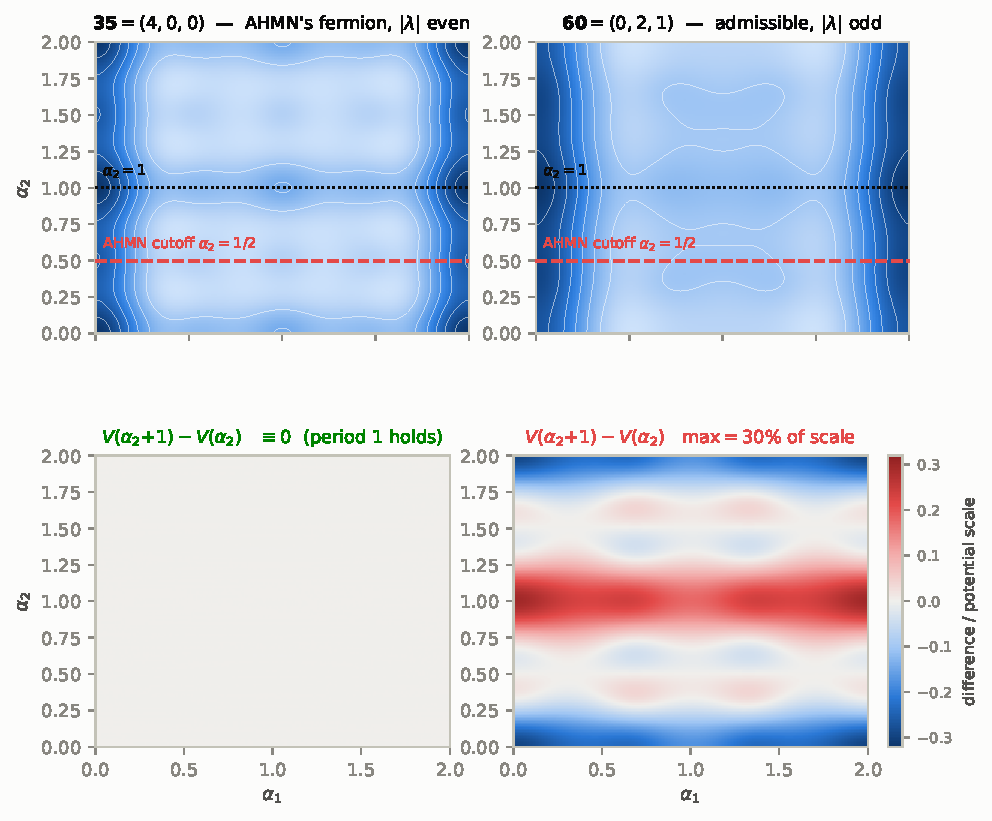
\includegraphics[width=\textwidth]{fig_domain.pdf}
\caption{The central claim, without algebra. \textbf{Top:} the one-loop Wilson-line potential
over the full period-$2$ torus, for AHMN's fermion (left) and for the smallest admissible
representation (right); the dashed line is the edge of the fundamental region
\eqref{eq:region} that the literature uses. \textbf{Bottom:} the direct test,
$V(\alpha_1,\alpha_2{+}1)-V(\alpha_1,\alpha_2)$ on the same scale. On the left it is
\emph{identically zero} --- flat grey, the periodicity holds and the half-domain is legal.
On the right it is a structured $30\%$ of the potential's own amplitude. Nothing about the
right-hand panel is smaller, subtler, or more numerical than the left; the symmetry is
simply absent, and every candidate representation that can host the Standard Model is on
that side.}
\label{fig:domain}
\end{figure}

The $\mathbf{35}$ is period-$1$ \emph{exactly}; every admissible representation violates it by
$2$--$30\%$ of the potential's own scale --- a physical amount, not numerical noise
(Figure~\ref{fig:domain}). The
reflection $\alpha_2\to-\alpha_2$ does survive in all nine. Hence for admissible
representations the fundamental region is $\alpha_2\in[0,1]$: exactly twice AHMN's.

\begin{corollary}\label{cor:domain}
The reduction \eqref{eq:region} does not transfer from AHMN's model to any
Standard-Model-admissible representation. A minimization for such a representation must scan
the full torus; a search restricted to the half-domain can return a boundary point that is
not a vacuum.
\end{corollary}

\paragraph{And no other identification rescues it.} Enlarging a fundamental domain invites
the obvious objection: perhaps some \emph{other} identification, not considered here, shrinks
it again. On a torus the natural candidates are the modular transformations, which act on the
Wilson-line phases by mixing the two cycles --- the same group that organizes the modular
flavour-symmetry programme~\cite{Feruglio,RatzEclectic}. We therefore measured, rather than
assumed, which lattice transformations $V$ actually respects. The surviving group is exactly
$\{\alpha_1\to\pm\alpha_1\}\times\{\alpha_2\to\pm\alpha_2\}$ together with the translations:
the reflections and $S^2=-\mathbf{1}$ hold to machine zero for every representation tested,
while $S$ itself, the exchange $\alpha_1\leftrightarrow\alpha_2$, and the shear
$\alpha_1\to\alpha_1+\alpha_2$ are all broken at order unity. This is what one should expect
from \eqref{eq:U}: $U_5=\mathbf{1}$ while $U_6\neq\mathbf{1}$, so the two cycles are
inequivalent and nothing that mixes them can survive the orbifold projection. The
consequence for us is that $\alpha_2\in[0,1]$ is not merely larger than \eqref{eq:region} ---
it is the correct and \emph{complete} fundamental region, with no further identification
available to reduce it.

One residual is worth flagging rather than interpreting. The shear
$\alpha_2\to\alpha_1+\alpha_2$ is broken, but by a margin that falls monotonically with the
dimension of the representation: $0.24$, $0.18$, $0.13$, $0.075$ and $0.027$ for the
$\mathbf{35}$, $\mathbf{60}$, $\mathbf{84}$, $\mathbf{216}$ and $\mathbf{360}$
respectively. Whether that is an
asymptotic recovery of a modular symmetry in the large-representation limit, or merely the
smoothing of the potential as more modes contribute, we do not know; a single monotone
sequence is not evidence, and we state it as an observation only.

This is not an erratum for~\cite{AHMN}, whose field content satisfies its own hypothesis. It
is a warning for everything downstream: the natural next step in this program --- putting a
realistic quark-hosting representation into the AHMN machinery --- silently loses a symmetry
that the machinery's conventions assume. We paid this ourselves. An earlier version of our
own naturalness ranking was computed on the half-domain, and its minimizer pinned to the
$\alpha_2=\tfrac12$ boundary for five of nine representations; we diagnosed it as an
implementation defect and fixed it numerically. It was not a defect. It was an inherited
symmetry that our representations do not have.

\emph{Established here:} the half-domain reduction inverts on the physical class, verified
on the potential itself. \emph{Left open:} what the admissible class gets \emph{instead} ---
the subject of the next section, and not what one would guess.

% ===================================================================
\section{What the notch buys: an exact decoupling}\label{sec:decoupling}
The odd-$m$ pairing buys periodicity. The even-$m$ notch buys something quite different, and
the difference is the reason a naturalness ranking in this class has been so hard to
stabilize.

The shape of what follows is familiar from a different context. Appelquist and Carazzone
proved that heavy states drop out of low-energy observables up to suppressed
corrections~\cite{AppelquistCarazzone}, and the lesson absorbed since is double-edged:
whatever is protected from an observable is also \emph{invisible} to it. A quantity that a
symmetry forbids from contributing cannot be measured by what it does not contribute to.
What we find below is a discrete, exact version of that trade. The notch does not suppress
the fermion representation's contribution to a particular observable; it annihilates it. And
the price is exactly the one Appelquist and Carazzone's readers learned to expect: that
observable can no longer tell one representation from another.

The leading Kaluza--Klein order of the $\alpha_2$-curvature at the half point is built
\emph{entirely} out of the even-$m$ imbalance
$\delta(m):=\mathrm{mult}(m,0)-\mathrm{mult}(m,1)$:
\begin{equation}\label{eq:Dstruct}
\mathcal D\;=\;\pi^2\Big(\sum_{m\equiv2\,(4)}m^2\delta(m)\;-\;\sum_{m\equiv0\,(4)}m^2\delta(m)\Big).
\end{equation}
But the notch is precisely the statement $\delta(m)=0$ for all even $m$. Therefore:

\begin{corollary}[Decoupling]\label{cor:decoupling}
For every Standard-Model-admissible representation, the fermion sector's contribution to
$\mathcal D$ vanishes identically. $\mathcal D$ reduces to the gauge sector alone --- the
same number for every admissible representation, independent of $(a,b,c)$.
\end{corollary}

Numerically, $\mathcal D=-27.6$ for all eight admissible representations, identical to the
digit, while the non-admissible $\mathbf{35}$, which breaks the notch, sits apart at
$-185.5$. This is the familiar shape of a conservation law: what makes the notch a clean
\emph{detector} of admissibility makes it blind as a \emph{discriminator} among admissible
representations.

\paragraph{A refuted inference, recorded deliberately.} It is tempting to conclude from
$\mathcal D<0$ uniformly that $\alpha_2=\tfrac12$ is a curvature ridge for every admissible
representation. That inference is false, and we record it because the failure is instructive.
Against the true curvature (converged, $K_{\max}=16$):

\begin{center}\footnotesize
\begin{tabular}{lccccccccc}
\toprule
\rowcolor{hdrblue}
\textcolor{white}{rep} & \textcolor{white}{$\mathbf{35}$} & \textcolor{white}{$\mathbf{60}$} &
\textcolor{white}{$\mathbf{84}$} & \textcolor{white}{$\mathbf{140}a$} & \textcolor{white}{$\mathbf{140}b$} &
\textcolor{white}{$\mathbf{216}$} & \textcolor{white}{$\mathbf{224}$} & \textcolor{white}{$\mathbf{280}$} &
\textcolor{white}{$\mathbf{360}$}\\
\midrule
$\mathcal D$ (leading order) & $-185.5$ & $-27.6$ & $-27.6$ & $-27.6$ & $-27.6$ & $-27.6$ & $-27.6$ & $-27.6$ & $-27.6$\\
\rowcolor{softgrey}
true $\partial^2_{\alpha_2}V$ at $\tfrac12$ & $-200.6$ & $+21.2$ & $-5.8$ & $-85.1$ & $-188.6$ & $+255.2$ & $-160.4$ & $+16.8$ & $+245.5$\\
sign agrees & yes & \textbf{no} & yes & yes & yes & \textbf{no} & yes & \textbf{no} & \textbf{no}\\
\bottomrule
\end{tabular}
\end{center}

The leading-order proxy mispredicts the sign in four of eight. It is right on the
$\mathbf{35}$ --- the one representation where the fermion sector dominates it, and the case
against which such a proxy is implicitly calibrated. It was validated in the only regime
where it works and then applied in the regime where the notch has removed its content.

\paragraph{The consequence that matters.} Putting the two together:

\begin{quote}
The notch does not fix the sign of the $\alpha_2$-curvature; it \emph{annihilates the
leading term}. For every admissible representation the leading Kaluza--Klein order is
degenerate --- identical, gauge-only. Everything that distinguishes one admissible
representation from another lives in the subleading terms.
\end{quote}

This explains from theory, rather than from post-mortem, why a naturalness ordering over this
class is delicate: the candidates are indistinguishable at leading order \emph{by a
theorem}, and the quantity that separates them is exactly the one a coarse minimization
resolves worst. Together with Corollary~\ref{cor:domain}, the two known failure modes of such
a computation are consequences of the same parity flip.

\emph{Established here:} an exact decoupling, and the structural origin of the fragility.
\emph{Left open:} the subleading structure itself --- which now has a target, since the
leading order is known in closed form to be a constant.

% ===================================================================
\section{Measuring the space instead of the point}\label{sec:basin}
Every fragility above comes from evaluating at a point: a minimizer pinned to a boundary, a
curvature read at that boundary, a Hessian taken by finite differences, a near-zero
eigenvalue in a flat direction. The one exact statement of this paper --- the notch --- is a
statement about the full Fourier content of $V$ over the torus. That asymmetry suggests
changing instrument.

For a quadratic well the sublevel set $S(\varepsilon)=\{V<V_{\min}+\varepsilon\Delta V\}$ is
an ellipse with semi-axes $\sqrt{2\varepsilon\Delta V/\lambda_i}$, and a uniform ellipse has
second-moment tensor $M_{ii}=a_i^2/4$. Both curvature eigenvalues therefore follow from an
\emph{integral} over the basin,
\begin{equation}
\lambda_i=\frac{\varepsilon\,\Delta V}{2\,M_{ii}},
\end{equation}
with no derivatives and no step size. Two corrections are required and both were found by
testing rather than by reasoning: $\varepsilon$ must lie in the quadratic regime (at
$\varepsilon=0.15$ the sublevel set covers $40$--$76\%$ of the torus and $M$ saturates
against the torus itself, reading a genuine $413{:}1$ anisotropy as $1.17{:}1$), and
$S(\varepsilon)$ must be restricted to the connected component of the global minimum, since
the torus carries symmetry-equivalent minima and an unrestricted set measures the separation
\emph{between} minima --- the signature being $\lambda\propto\varepsilon$ instead of a
plateau.

Corrected, the measure has a plateau at $\varepsilon\in[3\cdot10^{-4},10^{-3}]$ reproducing
the finite-difference Hessian for eight of nine representations. On the ninth ---
$(0,3,1)$, the one where finite differences are untrustworthy --- the drift under
$K_{\max}\!:\,4\to14$ falls from $68.9\%$ to $0.6\%$. Two facts established along the way are
worth recording: the vacuum \emph{location} is already converged at $K_{\max}=4$ (identical
to four decimals up to $K_{\max}=14$; the $\mathbf{35}$ lands at $(0.4360,0.2986)$ against
AHMN's quoted $(0.438,0.299)$, confirming the calibration), so under-convergence never
affected where the vacuum is, only the curvature there; and the low mode of $(0,3,1)$ is
genuinely \emph{anharmonic}, with no $\varepsilon$-plateau at all, so a quadratic mass is
simply the wrong descriptor for that direction rather than a hard-to-measure one.

\emph{Established here:} an integral replacement for the Hessian, validated where the Hessian
is trustworthy and stable where it is not. \emph{Left open:} the subleading ranking itself.

% ===================================================================
\section{A preflight, and who should run it}\label{sec:tool}
Part~I ended by packaging its Existence theorem as a reusable oracle rather than leaving it
as a claim about one model. The same is worth doing here, because
Corollary~\ref{cor:domain} is not a fact about $(3,\mathbf{60})$ --- it is a check that
anybody building on this class of construction should run \emph{before} spending computer
time.

\paragraph{What it is for.} The reduction \eqref{eq:region} is the kind of step that travels
as a convention. It appears once, is justified once for one field content, and is thereafter
inherited --- reasonably, since re-deriving every fundamental domain would make the
literature unreadable. The trouble is that its hypothesis is representation-dependent and
inverts on exactly the representations one would want to use next. A minimization run on the
halved region for such a representation does not fail loudly; it returns a boundary point
that looks like a vacuum. That failure mode is silent, which is why it deserves a tool
rather than a remark.

\paragraph{What it does.} \texttt{notch\_preflight.py} takes either Dynkin labels or an
explicit $(m,q)$ multiplicity table and reports which pairing the tower satisfies, which
fundamental region is therefore legal, and whether the representation can host a quark cell
at all. On labels it applies Corollary~\ref{cor:dichotomy} and Theorem~\ref{thm:Z} directly;
on a table it \emph{measures} both pairings rather than assuming either, so it remains valid
for spectra outside the $SU(4)$ setting where our theorem applies. Typical output:

\begin{center}\small
\begin{tabular}{ll}
\toprule
\rowcolor{hdrblue}
\textcolor{white}{\texttt{notch\_preflight.py 0 2 1}} & \textcolor{white}{\texttt{notch\_preflight.py 4 0 0}}\\
\midrule
centre charge: odd & centre charge: even\\
\rowcolor{softgrey}
tower pairs at: even $m$ & tower pairs at: odd $m$\\
odd-$m$ hypothesis: \textcolor{warmred}{\textbf{FAILS}} & odd-$m$ hypothesis: \textcolor{okgreen}{\textbf{HOLDS}}\\
\rowcolor{softgrey}
legal region: $\alpha_2\in[0,1]$ \textbf{(full torus)} & legal region: $\alpha_2\in[0,\tfrac12]$\\
hosts a quark cell: \textbf{yes} & hosts a quark cell: no\\
\bottomrule
\end{tabular}
\end{center}

\paragraph{Who should run it.} Anyone extending a gauge--Higgs orbifold model to a new
matter representation, before minimizing; anyone reusing a published fundamental domain with
different field content; and anyone who finds a minimizer settling repeatedly on a domain
boundary --- which, as \S\ref{sec:domain} records, is what a missing symmetry looks like from
the inside. The check costs nothing: it is one parity bit.

\emph{Established here:} the paper's operative consequence as a runnable check.
\emph{Left open:} the same question for other orbifold groups, where the alphabet in
\eqref{eq:D} changes and the dichotomy must be re-derived rather than reused --- exactly the
mistake this tool exists to prevent.

% ===================================================================
\section{Ledger}\label{sec:ledger}
As in Part~II we set out ownership item by item rather than in prose;
Table~\ref{tab:ledger} is that accounting.

\begin{table}[h]
\centering\small
\begin{tabular}{p{4.0cm}p{5.0cm}p{5.2cm}}
\toprule
\rowcolor{hdrblue}
\textcolor{white}{Item} & \textcolor{white}{Inherited (cite)} & \textcolor{white}{Ours}\\
\midrule
centre-charge congruence &
$\ZZ_4$ $n$-ality; fractional $Y$ locked to the centre~\cite{Hucks,Saller,Tong,Alonso,Slansky} &
nothing --- as in Part~II, we claim none of it\\
\midrule
\rowcolor{softgrey}
orbifold, twists $(m,q)$, one-loop potential, Eq.~\eqref{eq:region} &
AHMN~\cite{AHMN} &
the derivation of $(m,q)$ from the boundary conditions, and the multiplet reading of
AHMN's Table~1\\
\midrule
parity lemma~\ref{lem:parity} &
elementary (symmetry + homogeneity of $s_\lambda$) & presented as a remark, not a result\\
\midrule
\rowcolor{softgrey}
$D\equiv0$ mechanism &
$O(2n)$ associate/det-twist; Littlewood restriction; King modification rules~\cite{King71,Newell,Brauer,AyyerBehrend} &
the explicit arithmetic classification (Thm.~\ref{thm:Z}) and its Lean certificate\\
\midrule
the dichotomy, Cor.~\ref{cor:dichotomy} & --- & ours\\
\midrule
\rowcolor{softgrey}
inversion of \eqref{eq:region}, Cor.~\ref{cor:domain} & --- & ours, and verified on the potential directly\\
\midrule
decoupling, Cor.~\ref{cor:decoupling} & --- & ours\\
\bottomrule
\end{tabular}
\caption{What each result owes. The novelty of \S\ref{sec:degenerate} is a statement, not a
phenomenon and not a technique; the novelty of \S\S\ref{sec:domain}--\ref{sec:decoupling} is
the physics.}
\label{tab:ledger}
\end{table}

\paragraph{Where we looked.} For a general criterion deciding when a $GL(n)$ character
vanishes identically on $O(n)^-$ --- of which Theorem~\ref{thm:Z} would be a corollary --- we
read Koike--Terada~\cite{KoikeTerada}, King~\cite{King71b}, Littlewood~\cite{Littlewood58},
Fauser--Jarvis--King--Wybourne~\cite{FJKW}, Ayyer--Kumari~\cite{AyyerKumari},
Kumari~\cite{Kumari}, Ayyer--Behrend~\cite{AyyerBehrend} and Albion~\cite{Albion}, and found
none. Koike--Terada cannot contain one: they define $R(O(n))$ as a subring of $R(SO(n))$, and
since $V_\mu$ and $V_\mu\otimes\det$ restrict to the same $SO(n)$-irreducible the associate
involution is quotiented out before the question can be posed. One near neighbour deserves
explicit separation: Ayyer--Kumari's Example~2.16 states an $O(4)$ parity criterion at
$(x,-x)$, which looks identical to ours and is not --- their torus element has determinant
$+1$, the \emph{proper} component. Two classical sources remain unread and are flagged as
such: King's 1971 modification-rules paper in its own exposition, and Littlewood's book,
Ch.~XI.

% ===================================================================
\section{Reflections}\label{sec:reflections}
\paragraph{An inherited convention carries an unstated hypothesis.} Equation
\eqref{eq:region} travels as a convention --- a fundamental domain, the kind of thing one
copies without re-deriving. Its justifying hypothesis does not travel with it, and in this
case the hypothesis inverts exactly on the class one would want to use next. We suspect this
is not an isolated case in orbifold model building, where fundamental domains, $Z_2$
assignments and ``without loss of generality'' reductions are routinely inherited across
papers with different field content. The cheap protection is to carry the hypothesis as an
executable check rather than as a remark.

\paragraph{The centre as a constraint on the potential, not on the matter.} The shift in
viewpoint is easy to lose among the corollaries, so we state it bluntly.

For fifty years the centre of the gauge group has been used in one direction. Dirac's
quantization, 't~Hooft's phases, Hucks and Saller's reading of the Standard Model's own
$\ZZ_6$: in each the centre is a condition on \emph{which representations may exist}, or
carry which charges. Part~II used it that way too, and said so. The centre restricts matter.

What we have found is that in a gauge--Higgs construction the same invariant also restricts
the \emph{potential}. Not by making some contribution small: by removing an entire Fourier
sector of the Hosotani potential identically, for every representation of the wrong parity.
The Higgs in these models is a Wilson line; a period of Wilson line is a central gauge
transformation; so the centre acts on the Higgs sector as directly as it acts on the matter
sector, and its charge decides what can appear there. Figure~\ref{fig:spectrum} is that
statement drawn: for eight of nine representations an arithmetically specified sublattice of
harmonics is not small, it is empty.

We would put it this way. The centre charge has been read as a gate on matter. It is also a
gate on the potential, and the two gates open in opposite directions --- which is why a
condition that lets a representation host the Standard Model is the same condition that
denies its Wilson-line potential a symmetry the literature has been assuming.

\paragraph{A conjecture, stated so it can be killed.} The mechanism we can prove is
$SU(4)$-specific in its arithmetic but not in its logic, and it is more useful to say what we
expect than to stop at what we computed.

\begin{quote}
\emph{Conjecture (centre-parity selection, general form).} Let an orbifold gauge--Higgs model
have a Kaluza--Klein spectrum whose twist labels are captured by a character
$\chi_\lambda$ evaluated on an alphabet $A$, in the manner of \eqref{eq:D}. Suppose a unit
shift of a Wilson-line modulus carries $A$ to $\zeta\cdot A$ up to a Weyl element, for some
$\zeta$ in the centre of the gauge group, of order $d$. Then the harmonics of the one-loop
potential split into $d$ sectors labelled by the centre charge modulo $d$, and the sectors
on which $\zeta^{\,c(R)}\neq1$ are identically absent from the potential of a representation
$R$.
\end{quote}

We prove the case $d=2$, in the model where every ingredient can be computed exactly, and we
verify the structural precondition across $SU(N)$ below. What we have not done is exhibit a
second model, of different $d$, in which the sectors appear as predicted; that is the obvious
test and the obvious way to kill this. A $\ZZ_N$ orbifold with $N>2$, or a Wilson line whose
unit shift realizes a central element of order three, would settle it in one calculation.

\paragraph{Is this an accident of $SU(4)$?} It is the first question to ask of
\eqref{eq:principle}, and it has a sharp answer rather than a hopeful one.

The principle needs the shift to equal a central element \emph{up to Weyl}, which is the
multiset condition $-A=A|_{t\to-t}$ on the alphabet $A=\{\varepsilon_i\,t^{c_i}\}$, with
$\varepsilon_i=\pm1$ from the $\ZZ_2$ twist and $c_i$ the Wilson-line charge. Split the slots
by $c_i$. Those with $c_i=\pm1$ satisfy the condition automatically, since
$-\varepsilon t^{\pm1}$ and $\varepsilon(-1)^{\pm1}t^{\pm1}$ are the same monomial. Those
with $c_i=0$ do not: negation flips their sign and nothing in $t$ can undo it, so they must
pair off, a $+1$ against a $-1$. \emph{The Wilson-line-neutral slots must carry balanced
twist signs}, and in particular there must be an even number of them.

For a single Wilson-line direction that means $N-2$ even, hence $N$ even. A brute-force sweep
over every alphabet of this shape confirms it:

\begin{center}\small
\begin{tabular}{lcccccc}
\toprule
\rowcolor{hdrblue}
\textcolor{white}{$SU(N)$} & \textcolor{white}{$N{=}3$} & \textcolor{white}{$N{=}4$} &
\textcolor{white}{$N{=}5$} & \textcolor{white}{$N{=}6$} & \textcolor{white}{$N{=}7$} &
\textcolor{white}{$N{=}8$}\\
\midrule
alphabets admitting the rule & $0$ & $192$ & $0$ & $4880$ & $0$ & $134400$\\
\rowcolor{softgrey}
neutral slots when it holds & --- & $2$ & --- & $4$ & --- & $6$\\
verdict & none & \textbf{exists} & none & \textbf{exists} & none & \textbf{exists}\\
\bottomrule
\end{tabular}
\end{center}

So the mechanism is neither an accident nor universal: it lives on the even unitary groups,
and \textbf{$SU(4)$ is the smallest group that can carry it}. The odd groups are excluded for
a reason one can state in a sentence --- an odd number of spectator slots cannot pair its
twist signs --- and that reason is structural, not numerical.

Two honest limits on the sweep. It assumes the AHMN shape: one $\ZZ_2$ twist contributing
signs, and one Wilson-line direction with charges in $\{0,\pm1\}$. A $\ZZ_N$ orbifold, or a
Wilson line with higher charges, changes the condition --- the relevant central element then
need not have order two, and the congruence that appears would be modulo its order rather
than modulo $2$. We have not swept those, and we do not claim them.

\paragraph{The method is a shadow.} It is worth naming what was actually done, because the
same move is available elsewhere. Nothing in this paper studies an $SU(4)$ representation
directly. What it studies is a \emph{shadow}: the specialization
$D(t)=s_\lambda(1,-1,t,t^{-1})$ collapses a four-dimensional weight system onto a single
Laurent polynomial, and the orbifold is what chooses the wall to project onto --- the two
$\ZZ_2$ parities and the Wilson line fix the alphabet, and we do not get to pick it. Read
that way the results are statements about shadows. The dichotomy
(Corollary~\ref{cor:dichotomy}) says the shadow is always symmetric, with the centre charge
deciding about which axis. The notch says the shadow has holes, at arithmetically exact
positions --- and Figure~\ref{fig:spectrum} is those holes. The degenerate class
$\mathcal Z$ of Theorem~\ref{thm:Z} is the strangest of the three: those representations cast
\emph{no shadow at all} on this wall. They are not small --- $\mathcal Z$ contains
representations of every size --- and from here they are simply invisible, which is why the
physics never sees them and why they had to be classified by algebra rather than found by
inspection.

The practical moral is that the wall is chosen for you. A different orbifold projection is a
different alphabet in \eqref{eq:D}, hence a different shadow and a different dichotomy; that
is precisely why \S\ref{sec:tool} warns against reusing the result rather than re-deriving
it. What generalizes is not the answer but the question: given a compactification, ask what
specialization it imposes on the character, and read the physics off the shadow.

\paragraph{A gate can be a filter.} The picture that emerges is that the representation acts
as a \emph{filter} on the vacuum wave: $V(\alpha)$ is a Fourier series in the Wilson line,
the Kaluza--Klein sum is a Fourier transform on the hidden torus, and the multiplicity
spectrum of the representation decides which components pass. Corollary~\ref{cor:decoupling}
says that admissible representations are precisely those whose filter is blind at leading
order --- selecting a representation that can host the Standard Model automatically installs
a notch in its own Higgs potential. Whether that blindness is a nuisance or a design
principle (choose the representation to shape the filter) is the question we would most like
to answer next.

\paragraph{The leading order is a constant, so aim below it.} Because
Corollary~\ref{cor:decoupling} fixes the leading term in closed form, the naturalness problem
is now well posed rather than merely hard: compute the subleading structure with an analytic
gradient and explicit convergence control, against a leading order known to be degenerate.
That is a sharper task than making a minimizer more careful, and it is the first time there
has been a reason to expect it to be necessary.

% ===================================================================
\section{Conclusion}\label{sec:conclusion}
Part~II identified its first gate as classical and gave it away. This paper shows the gate was
doing more work than the sector it was found in, and the reason is one sentence: advancing the
Wilson line by one period is, up to a Weyl reflection, multiplication by the central element
$-\mathbf{1}$, so the centre acts on the Higgs sector as directly as it acts on the matter
sector. A representation answers with a single bit, and that bit decides which harmonics of
the Hosotani potential are permitted to exist at all. What has been read for fifty years as a
restriction on \emph{which representations may carry which charges} is also a restriction on
\emph{what the potential may contain}.

Concretely: the parity of the $\ZZ_4$ centre charge
--- equivalently $a+c$ --- decides which of two Kaluza--Klein twist pairings a representation
satisfies, and the two are mutually exclusive outside an explicitly classified degenerate
class. One of those pairings is the hypothesis under which the two-Higgs-doublet
gauge--Higgs literature halves its Wilson-line fundamental domain; the other is what every
Standard-Model-admissible representation has instead. The consequence is concrete and, we
believe, unavoidable for the program: the half-domain reduction does not transfer, the full
torus must be scanned, and the leading Kaluza--Klein order of the curvature at the half point
is representation-independent, so any ordering of candidates by naturalness is a statement
about subleading terms whether or not it is presented as one.

We claim none of the centre-charge congruence, exactly as before. What we claim is that it is
not only a gate on matter: it is a gate on the potential, and the two gates open in opposite
directions. From one witness, to the law of eligibility, to the discovery that the law's most
classical clause governs the sector it was never asked about --- that is the arc of the three
papers.

\paragraph{Data availability and reproducibility.} All scripts, weight data, Lean~4 sources
and figure-generation code are provided as ancillary files; no data beyond what they generate
underlies any claim here. Every number regenerates from the ancillary scripts: the
bialternant sweep for Theorem~\ref{thm:Z}, the Lean~4 source of Table~\ref{tab:lean}, the
$(m,q)$ derivation and multiplet-spreading check of \S\ref{sec:projection}, the direct
periodicity test of \S\ref{sec:domain}, the decoupling and curvature comparison of
\S\ref{sec:decoupling}, and the basin measure of \S\ref{sec:basin} with its $\varepsilon$
and $K_{\max}$ sweeps.

\begin{thebibliography}{99}
\bibitem{PartI} C.~Mar\'in, \emph{Anomaly- and Tadpole-Compatible Fermion Completion of
Six-Dimensional $SU(4)$ Gauge--Higgs Unification} (Part~I), Zenodo (2026),
DOI:\,10.5281/zenodo.21429144.
\bibitem{PartII} C.~Mar\'in, \emph{Three Gates to a Quark Generation} (Part~II), Zenodo
(2026), DOI:\,10.5281/zenodo.21432628.
\bibitem{SSSW} C.A.~Scrucca, M.~Serone, L.~Silvestrini, A.~Wulzer, \emph{Gauge-Higgs
Unification in Orbifold Models}, JHEP \textbf{02} (2004) 049, hep-th/0312267.
\bibitem{AHMN} K.~Akamatsu, T.~Hirose, N.~Maru, A.~Nago, \emph{Two Higgs Doublet Model from
Gauge--Higgs Unification in Six Dimensions}, arXiv:2603.05857.
\bibitem{Slansky} R.~Slansky, \emph{Group theory for unified model building},
Phys.\ Rept.\ \textbf{79} (1981) 1.
\bibitem{Hucks} J.~Hucks, \emph{Global structure of the standard model, anomalies, and
charge quantization}, Phys.\ Rev.\ D \textbf{43} (1991) 2709.
\bibitem{Saller} M.~Saller, \emph{The Central Correlations of Hypercharge, Isospin, Colour
and Chirality in the Standard Model}, Nuovo Cim.\ A \textbf{111} (1998) 1375,
arXiv:hep-th/9802112.
\bibitem{Tong} D.~Tong, \emph{Line Operators in the Standard Model}, JHEP \textbf{07}
(2017) 104, arXiv:1705.01853.
\bibitem{Alonso} R.~Alonso, D.~Dimakou, J.~West, \emph{Fractional-charge hadrons and
leptons to tell the Standard Model group apart}, arXiv:2404.03438.
\bibitem{Brauer} A.~Solymos, D.~Jakab, Z.~Zimbor\'as, \emph{Extendibility of Brauer states},
arXiv:2411.04597. (Prop.~1 and Thms.~5, 9 of App.~A give, in modern notation, the Littlewood
restriction rule, the $O(2k)$ self-associate fact, and the Newell--King modification rules.)
\bibitem{King71} R.C.~King, \emph{Modification Rules and Products of Irreducible
Representations of the Unitary, Orthogonal, and Symplectic Groups}, J.\ Math.\ Phys.\
\textbf{12} (1971) 1588.
\bibitem{King71b} R.C.~King, \emph{Branching rules for classical Lie groups using tensor and
spinor methods}, Can.\ J.\ Math.\ \textbf{23} (1971) 176.
\bibitem{Newell} M.J.~Newell, \emph{Modification rules for the orthogonal and symplectic
groups}, Proc.\ Roy.\ Irish Acad.\ \textbf{54} (1951) 153.
\bibitem{Littlewood58} D.E.~Littlewood, \emph{Products and plethysms of characters with
orthogonal, symplectic and symmetric groups}, Can.\ J.\ Math.\ \textbf{10} (1958) 17.
\bibitem{KoikeTerada} K.~Koike, I.~Terada, \emph{Young-diagrammatic methods for the
representation theory of the classical groups of type $B_n$, $C_n$, $D_n$},
J.\ Algebra \textbf{107} (1987) 466.
\bibitem{FJKW} B.~Fauser, P.D.~Jarvis, R.C.~King, B.G.~Wybourne, \emph{New branching rules
induced by plethysm}, J.\ Phys.\ A \textbf{39} (2006) 2611, arXiv:math-ph/0505037.
\bibitem{AyyerKumari} A.~Ayyer, N.~Kumari, \emph{Factorization of classical characters
twisted by roots of unity}, J.\ Algebra \textbf{609} (2022) 437, arXiv:2109.11310.
\bibitem{Kumari} N.~Kumari, \emph{Factorization of classical characters twisted by roots of
unity: II}, arXiv:2212.12477.
\bibitem{AyyerBehrend} A.~Ayyer, R.E.~Behrend, \emph{Factorization theorems for classical
group characters, with applications to alternating sign matrices and plane partitions},
J.\ Combin.\ Theory Ser.\ A \textbf{165} (2019) 78, arXiv:1804.04514.
\bibitem{Albion} S.P.~Albion, \emph{Universal characters twisted by roots of unity},
arXiv:2212.07343.
\bibitem{tHooft} G.~'t~Hooft, \emph{On the phase transition towards permanent quark
confinement}, Nucl.\ Phys.\ B \textbf{138} (1978) 1.
\bibitem{ScherkSchwarz} J.~Scherk, J.H.~Schwarz, \emph{Spontaneous breaking of supersymmetry
through dimensional reduction}, Phys.\ Lett.\ B \textbf{82} (1979) 60.
\bibitem{Manton} N.S.~Manton, \emph{A new six-dimensional approach to the Weinberg--Salam
model}, Nucl.\ Phys.\ B \textbf{158} (1979) 141.
\bibitem{Fairlie} D.B.~Fairlie, \emph{Higgs' fields and the determination of the Weinberg
angle}, Phys.\ Lett.\ B \textbf{82} (1979) 97.
\bibitem{Hosotani} Y.~Hosotani, \emph{Dynamical mass generation by compact extra
dimensions}, Phys.\ Lett.\ B \textbf{126} (1983) 309.
\bibitem{KawamuraGUT} Y.~Kawamura, \emph{Triplet-doublet splitting, proton stability and
extra dimension}, Prog.\ Theor.\ Phys.\ \textbf{105} (2001) 999, arXiv:hep-ph/0012125.
\bibitem{AppelquistCarazzone} T.~Appelquist, J.~Carazzone, \emph{Infrared singularities and
massive fields}, Phys.\ Rev.\ D \textbf{11} (1975) 2856.
\bibitem{Weyl} H.~Weyl, \emph{The Classical Groups: Their Invariants and Representations},
Princeton University Press (1939).
\bibitem{LittlewoodBook} D.E.~Littlewood, \emph{The Theory of Group Characters and Matrix
Representations of Groups}, 2nd ed., Oxford University Press (1950).
\bibitem{Murnaghan} F.D.~Murnaghan, \emph{The Theory of Group Representations}, Johns
Hopkins Press (1938).
\bibitem{HoweTanWillenbring} R.~Howe, E.-C.~Tan, J.F.~Willenbring, \emph{Stable branching
rules for classical symmetric pairs}, Trans.\ Amer.\ Math.\ Soc.\ \textbf{357} (2005) 1601,
arXiv:math/0311159.
\bibitem{CiucuKrattenthaler} M.~Ciucu, C.~Krattenthaler, \emph{A factorization theorem for
classical group characters, with applications to plane partitions and rhombus tilings},
arXiv:0812.1251.
\bibitem{Feruglio} F.~Feruglio, \emph{Are neutrino masses modular forms?}, in
\emph{From My Vast Repertoire: Guido Altarelli's Legacy}, World Scientific (2019) 227,
arXiv:1706.08749.
\bibitem{RatzEclectic} H.P.~Nilles, S.~Ramos-S\'anchez, P.K.S.~Vaudrevange, \emph{Eclectic
flavor groups}, JHEP \textbf{02} (2020) 045, arXiv:2001.01736; see also M.~Ratz et al.\ for
the orbifold-based development of modular flavour symmetry.
\end{thebibliography}
\end{document}
